% Created 2023-03-03 Fri 12:52
% Intended LaTeX compiler: pdflatex
\documentclass[11pt]{article}
\usepackage[utf8]{inputenc}
\usepackage[T1]{fontenc}
\usepackage{graphicx}
\usepackage{longtable}
\usepackage{wrapfig}
\usepackage{rotating}
\usepackage[normalem]{ulem}
\usepackage{amsmath}
\usepackage{amssymb}
\usepackage{capt-of}
\usepackage{hyperref}
\author{Raphaël Forment}
\date{\today}
\title{Sardine Documentation}
\hypersetup{
 pdfauthor={Raphaël Forment},
 pdftitle={Sardine Documentation},
 pdfkeywords={},
 pdfsubject={},
 pdfcreator={Emacs 28.2 (Org mode 9.6.1)}, 
 pdflang={English}}
\begin{document}

\maketitle
\tableofcontents

Sardine is a Live Coding Library for Python 3.10+. Control synthesizers through MIDI/OSC messages and interconnect audio/video softwares and/or sound engines. Explore algorithmic improvisation using a friendly syntax and a lightweight modular working environment.

\begin{center}
\begin{tabular}{lll}
\textbf{It's just Python!} & \textbf{Collaborative} & \textbf{Free/Open Source Software}\\[0pt]
\hline
Sardine is just timed Python. Customize your workflow using all the packages and libraries you like! Sardine can be extended for other purposes! Pattern your connected teapot! Crash in rhythm! & Sardine can be synchronized using the MIDI or the Link Protocol. Play with other musicians, sync your code with other instruments and music/video softwares. & Sardine is a collaborative effort! You can be a part of development by contributing with code, documentation or anything you'd like to share with the Sardine community.\\[0pt]
\end{tabular}
\end{center}

\section{Presentation}
\label{sec:org2001e78}
\subsection{{\bfseries\sffamily TODO} What is Sardine?}
\label{sec:org70dd7be}
\begin{center}
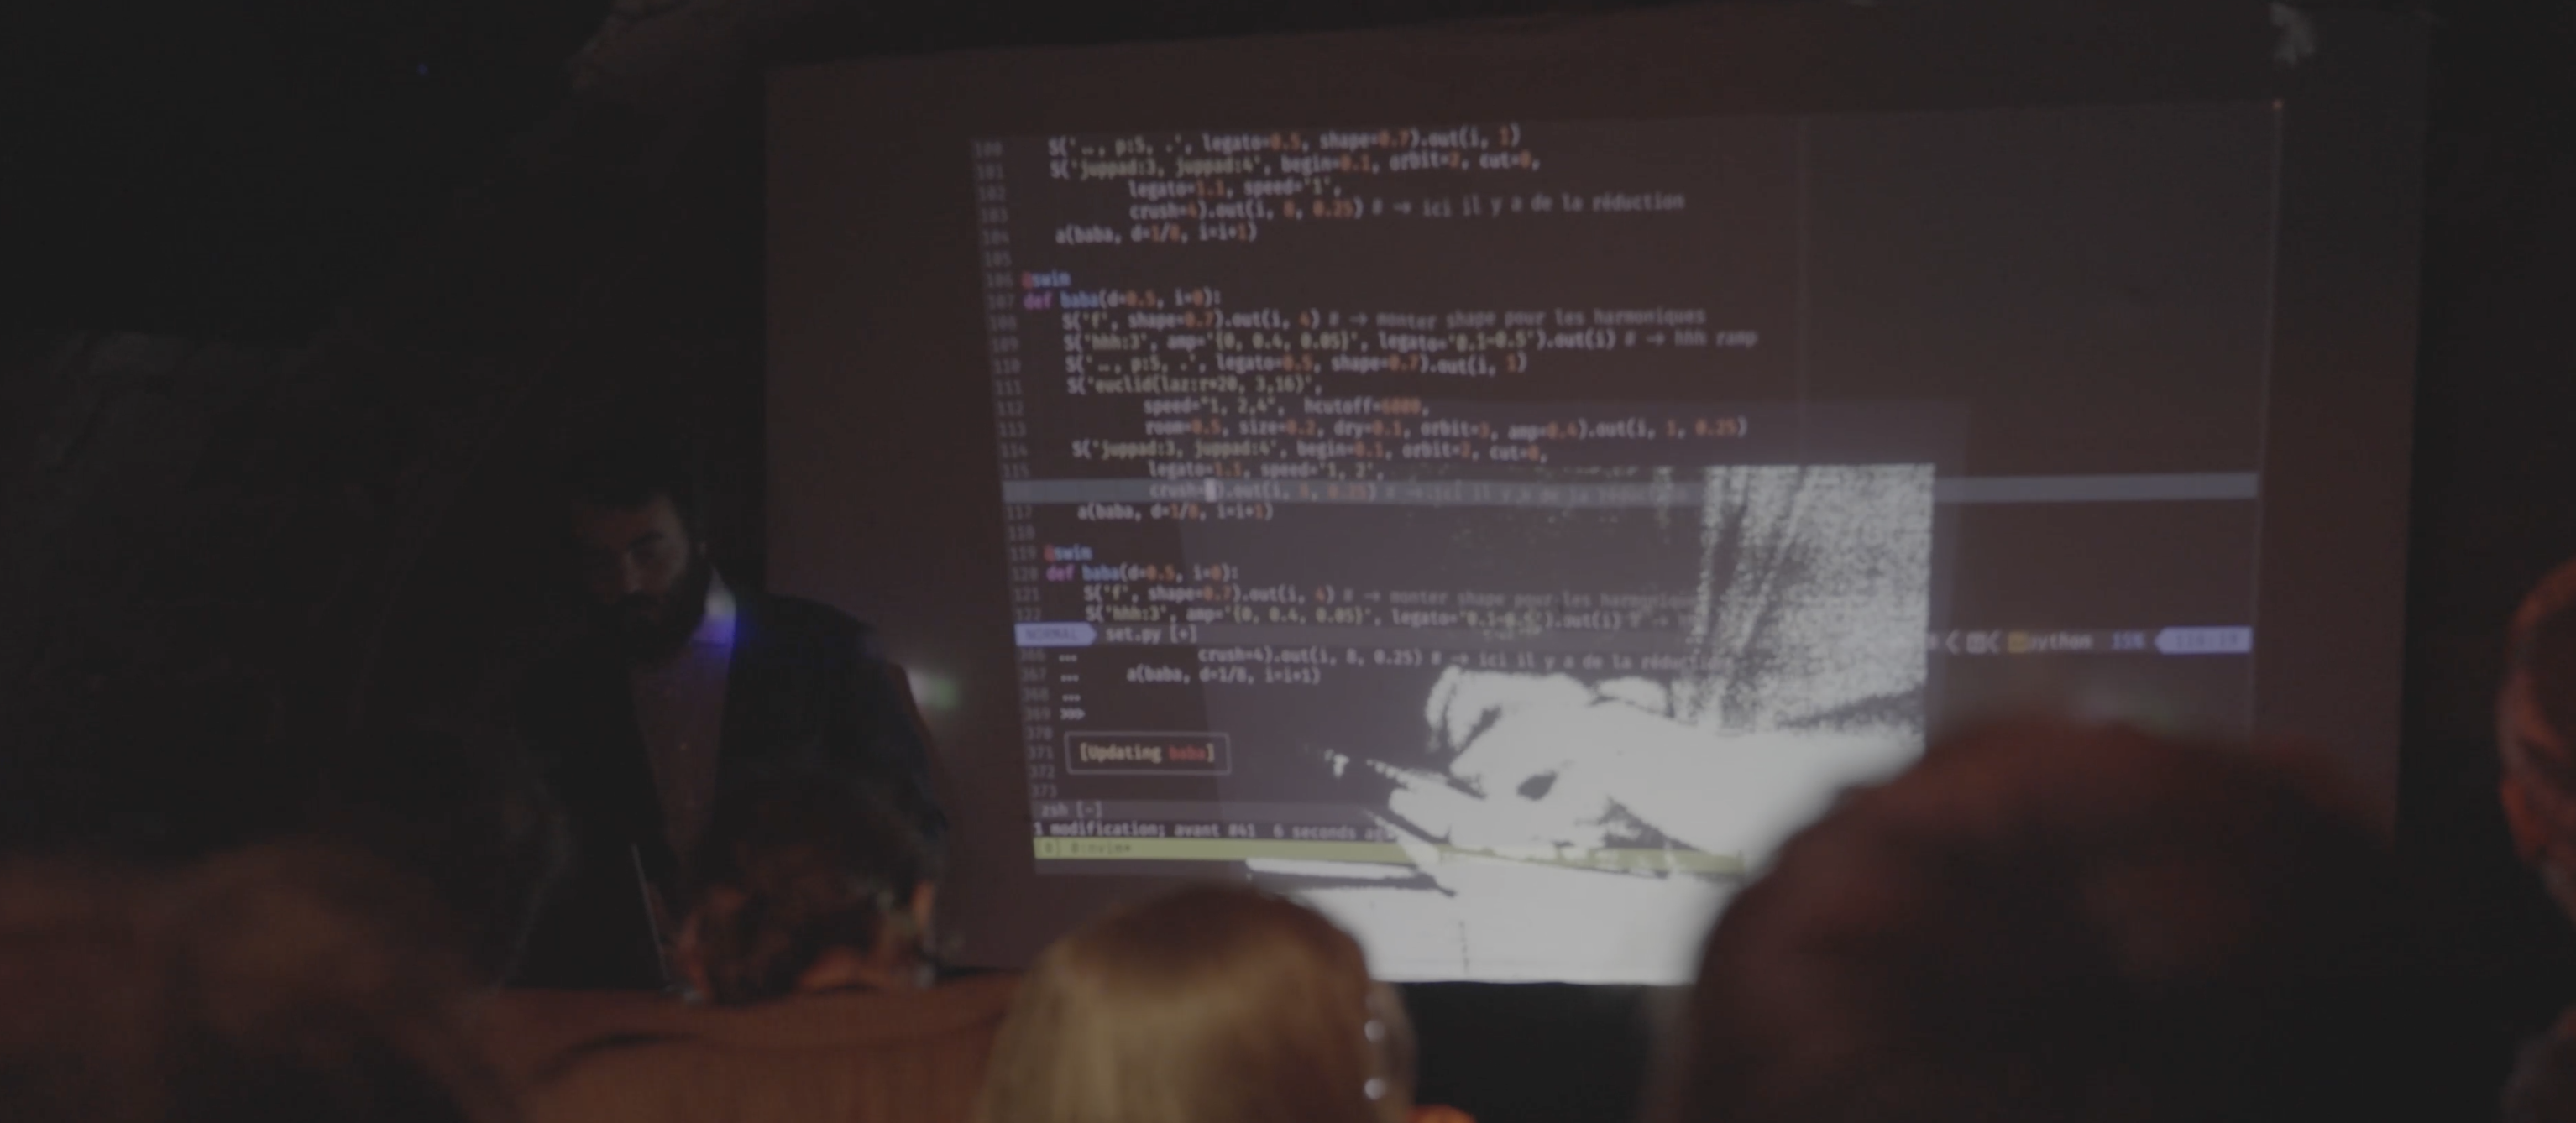
\includegraphics[width=.9\linewidth]{what_is_sardine.png}
\end{center}

Sardine is a \textbf{Python based musical instrument}. While it may look like a typical Python library, it is best described as a modular live coding environment. \textbf{Sardine} will allow you to sequence synthesizers, audio samples and various messages used by software or hardware audio/video equipment. \textbf{Sardine} is leveraging \textbf{Python} as a way to build powerful and terse algorithmic sequences that you can type fast while on stage. \textbf{Sardine} is also embedding multiple small languages (the more the merrier!) allowing you to do that even faster, and with style!

\textbf{Sardine} is using \textbf{Python} for its flexibility. \textbf{Python} is a very popular programming language for a good reason. It has a lot of different packages and it is very well supported pretty much everywhere :) You won't have any problem finding a good text editor or finding the right tools for the job.

\textbf{Sardine} is used by a small community of musicians and artists from France. You can find more in the \textbf{Demonstration} section or get in touch with us on social medias, \textbf{Discord}, etc\ldots{}

\begin{center}
\includesvg[width=.9\linewidth]{sardine_stack}
\end{center}

\subsection{{\bfseries\sffamily TODO} Community}
\label{sec:orgd38cab9}

There are multiple pages on the internet to share your new-found passion about \textbf{Sardine}:
\begin{itemize}
\item \href{https://discord.gg/aPgV7mSFZh}{Discord Server}: the most active place. Easy to reach me there as well :)
\item \href{https://github.com/Bubobubobubobubo/sardine}{Github Repository}: to check the latest news and to contribute to the code!
\end{itemize}

You can also find some \textbf{Sardine} related content by checking the \href{https://cookie.paris}{Cookie Collective} website.

\subsection{Showcase}
\label{sec:orgc36e27c}
\subsubsection{Example Code}
\label{sec:org803e69e}
\begin{enumerate}
\item Solstice
\label{sec:orgcf84fdd}

This piece was submitted by \textbf{BuboBubo}. This is a 20 minutes performance that I did for the \textbf{TidalCycles} annual solstice stream. Three of the four tracks were rapidly composed before the stream. I've tried to highlight some of the new features we have worked on for the \texttt{v.0.2.1}. I am sometimes playing additional keyboard on top of the code.

\begin{verbatim}
padcc = { 'timbre': {'control' : 18, 'chan': 2},
        'time': {'control' : 19, 'chan': 2},
        'metal': {'control' : 16, 'chan': 2},
        'fx': {'control' : 17, 'chan': 2}}
basscc = { 'timbre': {'control' : 18, 'chan': 0},
        'time': {'control' : 19, 'chan': 0},
        'cutoff': {'control' : 16, 'chan': 0},
        'fx': {'control' : 17, 'chan': 0}}
jupcc = { 'decay': {'control' : 81, 'chan': 1},
        'time': {'control' : 19, 'chan': 1},
        'cutoff': {'control' : 74, 'chan': 1},
        'resonance': {'control' : 71, 'chan': 1}}
dirt._ahead_amount = 0.4

#######################################################################
#█▀▀ █▀█ █▀▀ █▄░█ █▀▀ █░█   ▀█▀ █▀█ █░█ █▀▀ █░█   █▀ ▄▀█ █▀▄▀█ █▄▄ ▄▀█#
#█▀░ █▀▄ ██▄ █░▀█ █▄▄ █▀█   ░█░ █▄█ █▄█ █▄▄ █▀█   ▄█ █▀█ █░▀░█ █▄█ █▀█#
#######################################################################

PE >> d('long:3', cut=1, begin="[0.0:0.6,0.1]")

Pc >> d('ff:4!3, gg:12', cut=1, p=0.25, orbit=1, shape=0.5)

Pb >> d('f!7', cut=0, p=1, orbit=2, shape=0.5)

Pd >> d('g:10', p='.5, .5, .25', orbit=2, shape=0.5, speed='2,2,1!2,4')

Pb >> None
Pc >> None
Pc >> d('bip:rand*20', speed=2,
        cut=0, p=0.25, orbit=1, shape=0.5, hcutoff='[500:15000,1000]')

# ---

PE >> d('long:3', cut=1, begin="[0.0:0.6,0.1]")
Pc >> d('ff:4!3, gg:12', cut=1, p=0.25, orbit=1, shape=0.5)
Pb >> d('f!7', cut=0, p=1, orbit=2, shape=0.5)
Pd >> d('g:10', p='.5, .5, .25', orbit=2, shape=0.5, speed='2,2,1!2,4')
Pf >> d('bip:rand*50', speed=2, midinote='C5,C5,G5,A5',
        cut=1, p=0.25, orbit=1, shape=0.5)
Pg >> d('bip:rand*50', squiz=4, speed=1, midinote='C3,C4,G3,G4,A4,A5', shape=0.5,
        cut=1, p=0.25, orbit=1)

# ---

Pa >> None
Pb >> None
Pc >> None
Pd >> None

PE >> d('long:3', cut=1, begin="[0.0:0.6,0.1]")
Pc >> d('ff:4!3, gg:12', cut=1, p=0.25, orbit=1, shape=0.5)
Pb >> d('f!7', cut=0, p=1, orbit=2, shape=0.5)
Pd >> d('g:10', p='.5, .5, .25', orbit=2, shape=0.5, speed='2,2,1!2,4')
Pf >> d('bip:rand*50', speed=2, midinote='C5,C5,G5,G5',
        cut=1, p=0.25, orbit=1, shape=0.5)
Pg >> d('bip:rand*50', squiz=4, speed=1, midinote='C5@fifths', shape=0.5,
        cut=1, p=0.25, orbit=1)

Pa >> None
Pb >> None
Pc >> None
Pd >> None
PE >> d('long:3', cut=1, begin="[0.0:0.6,0.1]", speed='2!4,4!4')


PE >> d('long:3', cut=1, begin="[0.0:0.6,0.1]")
Pc >> d('ff:4!3, gg:12', cut=1, p=0.25, orbit=1, shape=0.5)
Pb >> d('f!7', cut=0, p=1, orbit=2, shape=0.5)
Pd >> d('g:10', p='.5, .5, .25', orbit=2, shape=0.5, speed='2,2,1!2,4')
Pf >> d('bip:rand*50', speed=2, midinote='C5,C5,G5,G5',
        cut=1, p=0.25, orbit=1, shape=0.5)
Pg >> d('bip:rand*50', squiz=4, speed=1, midinote='C5@fifths', shape=0.5,
        cut=1, p=0.25, orbit=1)

###################################################################
# █▀▀ ▄▀█ █▀█ █▀█ ▀█▀ ▀█▀ █▀▀   █ █▄░█ ▀█▀ █▀▀ █▀█ █░░ █░█ █▀▄ █▀▀#
# █▄▄ █▀█ █▀▄ █▄█ ░█░ ░█░ ██▄   █ █░▀█ ░█░ ██▄ █▀▄ █▄▄ █▄█ █▄▀ ██▄#
###################################################################

panic()

@swim
def baba(p=0.5, i=0):
    D('juppad:54, juppad:55', cutoff=2000, begin=0.1,
      orbit=2, cut=0, legato=1.1, i=i, d=8, r=0.25)
    again(baba, p=1/4, i=i+1)

@swim
def baba(p=0.5, i=0):
    D('juppad:54, juppad:55', cutoff=5000, begin=0.1,
      orbit=2, cut=0, legato=1.1, i=i, d=8, r=0.25)
    D('boop:rand*20', shape=0.4,
      midinote='G4|G5,Bb5,F6, G4|G5,Bb5,G6', i=i, r=0.25, d=2)
    D('boop:rand*40')
    again(baba, p=1/4, i=i+1)

@swim
def baba(p=0.5, i=0):
    # D('f', shape=0.4, i=i, d=4)
    # D('f:3', amp='[0:0.4,0.05]', legato='0.01~0.2', i=i)
    D('.., p:5, .', legato=0.5, shape=0.7, i=i, d=1)
    D('juppad:54, juppad:55', cutoff=5000, begin=0.1,
      orbit=2, cut=0, legato=1.1, i=i, d=8, r=0.25)
    D('.., p:6, ., .., p:3, ..', legato=0.5, shape=0.7, i=i)
    D('bip:rand*20', midinote='adisco((G|[G,G|Ab|G5])!2)', i=i, d=2)
    again(baba, p=1/4, i=i+1)

@swim
def baba(p=0.5, i=0):
    D('f, f, ..', shape=0.4, i=i, d=4)
    D('f:4', amp='[0:0.4, 0.05]', legato='0.1~0.5', i=i)
    D('.., p:5, .', legato=0.5, shape=0.7, i=i)
    D('juppad:54, juppad:55', cutoff=5000, begin=0.1,
      squiz=2, orbit=2, cut=0, legato=1.1, i=i, d=8, r=0.25)
    again(baba, p=1/4, i=i+1)

@swim
def baba(p=0.5, i=0):
    D('f', shape=0.4, i=i, d=4)
    D('f:8~12', speed='4~8', amp='[0:0.4, 0.05]', legato='0.1~0.5', i=i)
    D('.., p:5, .', legato=0.5, shape=0.7, i=i, d=1)
    D('laz:rand*20',
            speed="1, 2,4",  hcutoff='3000~6000',
            room=0.5, size=0.2, dry=0.1, orbit=3, amp=0.4, i=i, d=0.25)
    D('juppad:54, juppad:55', cutoff=5000, begin=0.1,
      squiz='0!4,2',
      orbit=2, cut=0, legato=1.1, i=i, d=8, r=1)
    again(baba, p=1/4, i=i+1)

@swim
def baba(p=0.5, i=0):
    # D('f', shape=0.4, i=i, d=4)
    # D('f:3', speed=4, amp='[0:0.4, 0.05]', legato='0.1~0.5', i=i)
    D('.., p:5, .', legato=0.5, shape=0.7, i=i)
    D('laz:rand*20',
            speed="1, 2,4",  hcutoff=6000,
            room=0.5, size=0.2, dry=0.1, orbit=3, amp=0.4, i=i, d=1, r=0.25)
    D('juppad:54, juppad:55', cutoff=5000, begin=0.1,
      pan='r', speed='1|2|4', leslie=1, lesliespeed=8,
      orbit=2, cut=0, legato=1.1, i=i, d=8, r=0.25)
    again(baba, p=1/4, i=i+1)

@swim
def baba(p=0.5, i=0):
    D('f', shape=0.4, i=i, d=4)
    D('.., p:5, .', legato=0.5, shape=0.7, i=i)
    D('conga:rand*20', speed="[1,2,4]/4", hcutoff='500~1000', shape=0.4,
            room=0.5, size=0.2, dry=0.1, orbit=3, amp=0.5, i=i, d=1, r=0.25)
    D('kit2:3', shape=0.5, i=i, d=8)
    D('., kit2:10, ., kit2:9!2', shape=0.5, i=i, d=2)
    again(baba, p=1/4, i=i+1)


@swim
def baba(p=0.5, i=0):
    D('f', shape=0.4, i=i, d=4)
    D('.., p:5, .', legato=0.5, shape=0.7, i=i)
    D('conga:rand*20', speed="[1,2,4]/4", hcutoff='500~1000', shape=0.4,
            room=0.5, size=0.2, dry=0.1, orbit=3, amp=0.5, i=i, d=1, r=0.25)
    D('conga:rand*20', speed="[1,2,4]/2", hcutoff='2000', shape=0.4,
            room=0.5, size=0.2, dry=0.1, orbit=3, amp=0.5, i=i, d=2, r=0.5)
    D('kit2:3', shape=0.5, i=i, d=8)
    D('., kit2:10, ., kit2:9!2', shape=0.5, i=i, d=2)
    again(baba, p=1/4, i=i+1)

# Ici on joue uniquement avec les percus et on lave les oreilles

@swim
def baba(p=0.5, i=0):
    D('f:3', amp='[0:0.2,0.01]', legato='0.1~0.5', i=i)
    D('.., p:(5|10), .', legato=0.5, i=i, d=1)
    D('m|c:[4:9]', legato=0.2, i=i, d='4!12, 3!12')
    D('jupbass:[1:100]', # -> lost into jupfx
            cutoff=3000, # ->
            shape=0.5,
            pan='sin($/40)', # -> X
            legato=0.2, # ->
            begin='r', i=i)
    again(baba, p=1/4, i=i+1)


@swim
def baba(p=0.5, i=0):
    D('a', shape=0.7, i=i, d=4)
    D('c', shape=0.7, i=i, d=3)
    D('d:7', orbit=3, room=0.2, size=0.8, dry=0.2, i=i, d=8)
    D('hhh:3', amp='[0:0.2, 0.01]', legato='0.1~0.5', i=i)
    D('f:3', amp='[0:0.2,0.01]', legato='0.1~0.5', i=i)
    D('.., p:(5|10), .', legato=0.5, i=i, d=1)
    D('m|c:[4:9]', legato=0.2, i=i, d='4!12, 3!12')
    D('jupbass:[1:100]', # -> lost into jupfx
            cutoff=3000, # ->
            shape=0.5,
            pan='sin($/40)', # -> X
            legato=0.2, # ->
            begin='r', i=i)
    again(baba, p=1/4, i=i+1)

panic()
D('girls:2')


#####################################################################
# █▀▀ █▀█ █▀▄▀█ █▀█ █░█ ▀█▀ █▀▀ █▀█   █░░ ▄▀█ █▀▄▀█ █▀▀ █▄░█ ▀█▀ █▀█#
# █▄▄ █▄█ █░▀░█ █▀▀ █▄█ ░█░ ██▄ █▀▄   █▄▄ █▀█ █░▀░█ ██▄ █░▀█ ░█░ █▄█#
#####################################################################

@swim
def structure(p=0.5, i=0):
    N("C2,C3", chan=2, vel=120, i=i)
    N("G5,G4", chan=2, vel=120, i=i, r=0.25/4)
    N("[G6]-[0:12]", chan=2, vel=120, i=i, r=0.25/2)
    CC(**jupcc['cutoff'], value=100)
    CC(**jupcc['decay'], value=80)
    N("[G6]-[0:12]", chan=1, vel=120, i=i, r=0.25/2)
    again(structure, p=0.5, i=i+1)

@swim
def structure(p=0.5, i=0):
    N("C2,C3", chan=2, vel=120, i=i)
    N("G5,G4", chan=2, vel=120, i=i, r=0.25/4)
    N("[G6|D5]-[0:12]", chan=2, vel=120, i=i, r=0.25/2)
    again(structure, p=0.5, i=i+1)

@swim
def structure(p=0.5, i=0):
    CC(**padcc['timbre'], value='50~120')
    N("C2,C3", chan=2, vel=120, i=i)
    N("G5,G4", chan=2, vel=120, i=i, r=0.25/4)
    N("[G6]-[0:12]", chan=2, vel=120, i=i, r=0.25/2)
    again(structure, p=0.5, i=i+1)

@swim
def structure(p=0.5, i=0):
    N("C2,C3", chan=2, vel=120, i=i)
    N("G5,G4", chan=2, vel=120, i=i, r=0.25/4)
    N("[G6]-[0:12]", chan=2, vel=120, i=i, r=0.25/2)
    N("[G7]-[0:12]", chan=2, vel=120, i=i, r=0.25/1)
    again(structure, p=0.5, i=i+1)

@swim
def structure(p=0.5, i=0):
    CC(**padcc['timbre'], value='(90~100)-10') # go down
    N("C2,C3", chan=2, vel=120, i=i)
    N("G5,G4", chan=2, vel=120, i=i, r=0.25/4) # middle voice
    N("Eb4, F4, G4", chan=2, vel='50~100', i=i, r=0.25/2)
    N("pal(C|C5|C6@minor)", d=2,
      chan=2, vel='50~100', i=i, r=0.25/2)
    again(structure, p=0.5, i=i+1)

@swim
def structure(p=0.5, i=0):
    CC(**padcc['timbre'], value='(70~110)') # go down
    N("C2,C3", chan=2, vel=120, i=i)
    N("G5,G4", chan=2, vel=120, i=i, r=0.25/4)
    N("Eb4, F4, G4", chan=2, vel='50~100', i=i, r=0.25/2)
    N("pal(C|C5|C6@minor)", d=2,
      chan=2, vel='50~100', i=i, r=0.25/2)
    CC(**basscc['timbre'], value='rand*127')
    CC(**basscc['fx'], value='80')
    CC(**basscc['cutoff'], value='[1:127,20]')
    N("disco(pal(C3|C5|C4@minor))", d=1,
      chan=0, vel='(50~100)-30', i=i, r=0.25)
    again(structure, p=0.5, i=i+1)

@swim
def structure(p=0.5, i=0):
    N("C2,C3", chan=2, vel=120, i=i)
    N("G5,G4", chan=2, vel=120, i=i, r=0.25/4)
    N("Eb4, F4, G4", chan=2, vel='50~100', i=i, r=0.25/2)
    CC(**basscc['cutoff'], value=127, i=i)
    N("pal(C|C5|C6@minor)", d=2,
      chan=2, vel='50~100', i=i, r=0.25/2)
    N("disco(pal(C3|C5|C4@minor))", d=1,
      chan=0, vel='50~100', i=i, r=0.25)
    D('ff', d='3, 3, 2', i=i, cutoff=2500)
    D('s, u, n, d, o, w, n', d='3, 3, 2', i=i, p=0.5)
    D('kk:2~8, bb:1~9', legato=0.2, d='2, 3, 1!4', i=i,
      speed='0.25, 0.5!5, 1!8')
    again(structure, p=0.5, i=i+1)


@swim
def structure(p=0.5, i=0):
    N("C2,C3", chan=2, vel=120, i=i)
    N("G5,G4", chan=2, vel=120, i=i, r=0.25/4)
    N("Eb4, F4, G4", chan=2, vel='50~100', i=i, r=0.25/2)
    CC(**basscc[pick('timbre', 'cutoff')], value='20~120', i=i)
    CC(**basscc[pick('time')], value='20', i=i)
    N("pal(C|C5|C6@minor)", d=2,
      chan=2, vel='50~100', i=i, r=0.25/2)
    N("disco(pal(C4|C6|C5@minor))", d=1,
      chan=0, vel='50~100', i=i, r=0.25)
    D('ff', d='3, 3, 2', i=i, cutoff=2500)
    D('s, u, n, d, o, w, n', d='3, 3, 2', i=i, p=0.5)
    D('kk:2~8, bb:1~9', legato=0.2, d='2, 3, 1!4', i=i,
      speed='0.25, 0.5!5, 1!8')
    again(structure, p=0.5, i=i+1)

Pb >> d('g,o,o,d,b,y,e,t,r,a,c,k', d='1', p=0.5, orbit=2, cut=0)

@swim
def structure(p=0.5, i=0):
    N("C2,C3, F2, F3", chan=2, vel=120, i=i)
    N("G5,G4, Ab5, Ab4", chan=2, vel=120, i=i, r=0.25/4)
    N("Eb4, F4, G4, Eb4, Eb5, Eb4, Eb5", chan=2, vel='50~100', i=i, r=0.25/2)
    N("pal(F|F5|G6@minor)", d=2,
      chan=2, vel='50~100', i=i, r=0.25/2)
    again(structure, p=0.5, i=i+1)


Pc >> d('s, u, n, d, o, w, n', d='3, 3, 2', p='0.25!16, 0.5!4', orbit=3, cut=1, speed='2,4')

@swim
def structure(p=0.5, i=0):
    N("pal(F|F4|G3@minor)", d=2,
      chan=2, vel='100~120', i=i, r=0.25/2)
    N("pal(F|F5|G6@minor)", d=2,
      chan=2, vel='100~120', i=i, r=0.25/2)
    again(structure, p=0.5, i=i+1)

############################################################
# IDEE POUR UN TROISIEME MORCEAU
############################################################

silence(structure)
Pc >> None
@swim(snap=0)
def baba(p=0.5, i=0):
    D('ff', i=i, d=4, shape=0.5)
    D('s:[1:20]', i=i, d=3, speed='1|1|2|4', legato=0.4, pan='r')
    D('l:[1:20]', i=i, d=2, speed='1|1|2|4', legato=0.2, pan='r')
    D('jupfx:[0:20]', midinote='rev(C3, Eb3, G, Bb4|Bb5)',
      room=0.5, size=0.21, dry=0.12, orbit=3, amp=0.25,
      i=i, d=2, speed='1|1|2|4', legato=0.08, pan='r')
    again(baba, p=0.25, i=i+1)


Pb >> None
@swim(snap=0)
def baba(p=0.5, i=0):
    D('long', orbit=3, cut=1, begin='r', i=i)
    D('ff', i=i, d=4)
    D('kit2:[1,20]', legato=0.1, i=i, d='3!32, 4!16', speed='1,2')
    again(baba, p=0.25, i=i+1)


@swim(snap=0)
def baba(p=0.5, i=0):
    D('ulh:60', orbit=3, cut=1, begin='r', i=i)
    D('ff', i=i, d=4)
    D('ff:9', i=i, d=8, orbit=2)
    if sometimes():
        D('ff:rand*40', i=i, d=2, orbit=2, legato=0.1)
    else:
        D('bb|gg:rand*40', speed='<1,2>,4', i=i, d=1, orbit=2, legato='0.01~0.2')
    D('kit2:[1,20]', legato=0.1, i=i, d='3!32, 4!16', speed='1,2')
    again(baba, p=0.25, i=i+1)
# Change p to 2, I don't know why but it is working

panic()


##################################################################
# █░█ █▀█ █░░ ▄▀█ █ █░░ █░░ █▀▀   █▀▄ █▀▀   █▄▄ █▀█ █▀▀ █▀ █▀ █▀▀#
# ▀▄▀ █▄█ █▄▄ █▀█ █ █▄▄ █▄▄ ██▄   █▄▀ ██▄   █▄█ █▀▄ ██▄ ▄█ ▄█ ██▄#
##################################################################

Pa >> d('juppad:12|51', begin='r', amp=0.20, speed='1', legato=4,
        room=0.5, orbit=3, dry=0.2, size=0.8,
        midinote='Do,Fa,Ab3,Eb4', cutoff=4000)

Pb >> d('bip:rand*50', begin='0,0.2,0.5', amp=0.45, speed='2',
        room=0.5, orbit=3, dry=0.2, size=0.8,
        legato=0.18, midinote='adisco(Do,Fa,Ab3,Eb4)', cutoff=8000, p=0.5)

Pd >> d('ff:4', shape=0.5, speed=1, p=0.5, cutoff='[200:2000,100]', amp=0.5)


Pa >> d('juppad:12|51', begin='r', amp=0.20, speed='1', legato=4,
        room=0.5, orbit=3, dry=0.2, size=0.8,
        midinote='Do,Fa,Ab3,Eb4', cutoff=4000)
Pb >> d('bip:rand*50', begin='0,0.2,0.5', amp=0.45, speed='2',
        room=0.5, orbit=3, dry=0.2, size=0.8,
        legato=0.18, midinote='adisco(Do,Fa,Ab3,Eb4)', cutoff=8000, p=0.5)
Pc >> d('ff', shape=0.5, speed=1, p=1, cutoff='[2000:5000,100]')
Pc >> d('nn:4~8', legato=0.2,
        shape=0.5, speed='1,2', p=0.5, cutoff='[2000:5000,100]')
Pe >> d('ff', shape=0.5, speed=1, p=2, cutoff='[200:2000,100]')

Pc >> d('[f,i,s,h,e,s]:[1:20]', shape=0.5, p=0.5, legato=0.02, pan='r')
Pd >> d('euclid([gg:rand*20]!8, 5,8)', shape=0.5, speed=4,
        p=0.5, cutoff='5000', resonance='0.1,0.2')

Pb >> None # d('j, a, j, a', orbit=2, p='1,0.5')
Pc >> None # d('f, l, o, w, e, e:rand*4', shape=0.5)
Pd >> None # d('bb:5~6', p='0.25, 0.125', legato=0.05)

panic()
\end{verbatim}

\item Zorba in Belleville
\label{sec:org9978337}

This code is taken from an algorave that took place at the \textbf{Zorba} (Belleville, Paris) in early november (2022). It is a very straightforward dance oriented performance that plays a lot with simple audio sample manipulations. As stated in the opening banner, this performance was meant to test the stability of \textbf{Sardine} after introducing new features and control mechanisms. Everything lives in the baba function, meaning that you only need to keep track one function during the whole performance.

Sounds are extracted from a very heavy sound library, lazy-loaded when needed. This is how I like to make music, extracting a lof of raw audio files from my hard disk :)

\begin{verbatim}
# ██████████████████████████████████████████████████████████████████████████████████████████████████████████████████
# █░░░░░░░░░░░░░░█░░░░░░░░░░░░░░█░░░░░░░░░░░░░░░░███░░░░░░░░░░░░███░░░░░░░░░░█░░░░░░██████████░░░░░░█░░░░░░░░░░░░░░█
# █░░▄▀▄▀▄▀▄▀▄▀░░█░░▄▀▄▀▄▀▄▀▄▀░░█░░▄▀▄▀▄▀▄▀▄▀▄▀░░███░░▄▀▄▀▄▀▄▀░░░░█░░▄▀▄▀▄▀░░█░░▄▀░░░░░░░░░░██░░▄▀░░█░░▄▀▄▀▄▀▄▀▄▀░░█
# █░░▄▀░░░░░░░░░░█░░▄▀░░░░░░▄▀░░█░░▄▀░░░░░░░░▄▀░░███░░▄▀░░░░▄▀▄▀░░█░░░░▄▀░░░░█░░▄▀▄▀▄▀▄▀▄▀░░██░░▄▀░░█░░▄▀░░░░░░░░░░█
# █░░▄▀░░█████████░░▄▀░░██░░▄▀░░█░░▄▀░░████░░▄▀░░███░░▄▀░░██░░▄▀░░███░░▄▀░░███░░▄▀░░░░░░▄▀░░██░░▄▀░░█░░▄▀░░█████████
# █░░▄▀░░░░░░░░░░█░░▄▀░░░░░░▄▀░░█░░▄▀░░░░░░░░▄▀░░███░░▄▀░░██░░▄▀░░███░░▄▀░░███░░▄▀░░██░░▄▀░░██░░▄▀░░█░░▄▀░░░░░░░░░░█
# █░░▄▀▄▀▄▀▄▀▄▀░░█░░▄▀▄▀▄▀▄▀▄▀░░█░░▄▀▄▀▄▀▄▀▄▀▄▀░░███░░▄▀░░██░░▄▀░░███░░▄▀░░███░░▄▀░░██░░▄▀░░██░░▄▀░░█░░▄▀▄▀▄▀▄▀▄▀░░█
# █░░░░░░░░░░▄▀░░█░░▄▀░░░░░░▄▀░░█░░▄▀░░░░░░▄▀░░░░███░░▄▀░░██░░▄▀░░███░░▄▀░░███░░▄▀░░██░░▄▀░░██░░▄▀░░█░░▄▀░░░░░░░░░░█
# █████████░░▄▀░░█░░▄▀░░██░░▄▀░░█░░▄▀░░██░░▄▀░░█████░░▄▀░░██░░▄▀░░███░░▄▀░░███░░▄▀░░██░░▄▀░░░░░░▄▀░░█░░▄▀░░█████████
# █░░░░░░░░░░▄▀░░█░░▄▀░░██░░▄▀░░█░░▄▀░░██░░▄▀░░░░░░█░░▄▀░░░░▄▀▄▀░░█░░░░▄▀░░░░█░░▄▀░░██░░▄▀▄▀▄▀▄▀▄▀░░█░░▄▀░░░░░░░░░░█
# █░░▄▀▄▀▄▀▄▀▄▀░░█░░▄▀░░██░░▄▀░░█░░▄▀░░██░░▄▀▄▀▄▀░░█░░▄▀▄▀▄▀▄▀░░░░█░░▄▀▄▀▄▀░░█░░▄▀░░██░░░░░░░░░░▄▀░░█░░▄▀▄▀▄▀▄▀▄▀░░█
# █░░░░░░░░░░░░░░█░░░░░░██░░░░░░█░░░░░░██░░░░░░░░░░█░░░░░░░░░░░░███░░░░░░░░░░█░░░░░░██████████░░░░░░█░░░░░░░░░░░░░░█
# ██████████████████████████████████████████████████████████████████████████████████████████████████████████████████

# █▀▀ █▀█ ▄▀█ █▀ █░█   ▀█▀ █▀▀ █▀ ▀█▀   █░█ █▀▀ █▀█ █▀ █ █▀█ █▄░█   ▄▀█ █░░ █▀█ █░█ ▄▀█   █▀█ ░ █▀█ █▀█ █▀█ █▀█ ▄█
# █▄▄ █▀▄ █▀█ ▄█ █▀█   ░█░ ██▄ ▄█ ░█░   ▀▄▀ ██▄ █▀▄ ▄█ █ █▄█ █░▀█   █▀█ █▄▄ █▀▀ █▀█ █▀█   █▄█ ▄ █▄█ █▄█ █▄█ █▄█ ░█

# @@@@@@@@@@@@@@@@@@@@@@@@@@@&&@@@@@@@@@@@@@@@@@@@@@@@@@@@@@@@@@@@@@@@@@@@@@@@@@@@@@@@@@@@@@@@@@@@@@@@@@@@@@@@@@@@@@@
# @@@@@@@@@@@@@@@@@....,.....,..,,,,,,,,,,,,,*(&@@@@@@@@@@@@@@@@@@@@@@@@@@@@@@@@@@@@@@@@@@@@@@@@@@@@@@@@@@@@@@@@@@@@@
# @@@@@@@@@@@@&.,,,,/*//////////**,*.*,*..,***,,,,**********/(%@@@@@@@@@@@@@@@@@@@@@@@@@@@@@@@@@@@@@@@@@@@@@@@@@@@@@@
# @@@@@@@@@@(..,*//**/***,,,,,(%((%%,/,%%%%(****,,.,,********,,,*/*/*****///(%@@@@@@@@@@@@@@@@@@@@@@@@@@@@@@@@@@@@@@@
# @@@@@@@@@ .,(/////*,,,,,,,/%%%(*.((,/%%(/.((/%/%//,//,/#%(*****************,,*****///////(&@@@@@@@@@@@@@@@@@@@@@@@@
# @@@@@@@@ ./(//*,*,,**,,,,,,,,,,*,*,,**,*/#%%%%%,*#(*(,,(*%(,(*,/*(%(#,/%%/****************,*//*//****/&@@@@@@@@@@@@
# @@@@@@@ .(##***,*,,,,,,,,,,,,,,,,,,,,,*,*,,****,*,****,*(%%%/##/(%,./*//(%(,(%(./((/,*%**************.,****%@@@@@@@
# @@@@@@.*///*********,*,**,,*,,,,,,,%%%%%((#%%%%%,,(%%%%%%%%%%%##%%#,,**/%&%%(/,&(,((/#%%%*,,,,,,,,,,,,,,,..***(@@@@
# @@@@@%/**/*****,,***,,,,,,,,,,,%%%%##/##%%%%%%%%%%%#((**###%%%%####%#####%#(,,********/#%***,,,,,,,,,,,,,,,,.,**/@@
# @@@@@,/**,**************,,,,,*%%%/.((*%*/,/((*#./*. .. ..*,/(##/*,,###*/#/(#%%%#(#,*,#%%%%%%%%%/,,*,,,,,,,,,,..***@
# @@@@ ,/**********,*******,,,,*,% #*,,//#%(.#*,,**#,(##(/**##%##%##/,/#%(//(//,.(#(#%#((,#%%##*##%%%,,,,,,,,,,,. ***
# @@@ .,///*******,*,*,**,,**,,*,,*./ /((..((/(%,,/#(/(/*,*#,.*#/###%%##/**/(/(/.(//%%%%%/###%##,,,%%%***,,,,,,.. .**
# @@@...////*************,***,,,/(((((*.(., #*(  *(..#/(/*(///(##(#(####(/#(*##%(/((%%%%%%%/((#%%%%%%%#***,,,**,   ,*
# @@,..../(//********,,***,,,***(((((( ((*((,,##,,,/###(//*(##((((((#(,       ,(%%#%%,.,(####%###,/%&******,*,*,   .(
# @@*/.,..*(*/***********,*,,*,,,,,**(.((.(((((((((**,(%%%%%%%%###########(*//(#((//*/. *,/(#%##,.,******,**,*,,   ,%
# @@,/*,*.,..(***************,,*,,,*,#*&(**(,* ((  .(((((..((((/********,,*,****/((((((,***********************,   *(
# @/,*/**,,*,,...,*,,*,*,..,,*,,,,,,*,*,**,(#&(,*,/((./(( (( /(. ...(((*../( (#((((((((((**********************  .*#,
# @, *//********/.,,.........,,,,,,,,,,*,,..,,,**,,**##(%&#*****/((#(((((((((((/*,***************************,...**%#
# @% ,*/******//////////**/****,.,,.........,,**/*,,,,,,,,,,,*,*******,************************************,.. **,#,@
# @@* .********/*///////////*/////////*********,,,,,,***//*//////***,*,,,,,,****************************,... ,***/#/@
# @@@#/..********///////////**/*,*,/#.//////////////**********,,.,,**********//*,,,,,,,.,***********,.....,*/*,*(#(&@
# @@@@@&(*,,******///////./,//**/.**//////,/***,/#,,//**,/.////////******/***,,..,,*,...,,**/*,,**,*//*/*****/((#%*@@
# @@@@@@@@%/(/,,,***///////*,,**/**////,**/*/,,**////**///***./*//.*/////////////*******/*,,******,,*//#/(//(((##*%@@
# @@@@@@@@@@@@@((/(((((/*,,,**//****///**,*//****///***.*//**////***////*(%%##%%/&&&///////////////(((((((((((###*@@@
# @@@@@@@@@@@@@@@@@@@@@@&#/(#####(((//*,,,,**/***//******,,***///**./*/**%%&&&###((&&%**//////////(((((((((((((/*@@@@
# @@@@@@@@@@@@@@@@@@@@@@@@@@@@@@@@@@@@&#/(####((((/**,,,,**/////****////****/%###%/%&***////////(((((((((((((/,(@@@@@
# @@@@@@@@@@@@@@@@@@@@@@@@@@@@@@@@@@@@@@@@@@@@@@@@@@&#/#####(((/(/*,,,,***///****///****/////////(((((((((/**(&@@@@@@
# @@@@@@@@@@@@@@@@@@@@@@@@@@@@@@@@@@@@@@@@@@@@@@@@@@@@@@@@@@@@@@@@&(/#####(((((/*,,,******///////((((//**#(%@@@@@@@@@
# @@@@@@@@@@@@@@@@@@@@@@@@@@@@@@@@@@@@@@@@@@@@@@@@@@@@@@@@@@@@@@@@@@@@@@@@@@@@@@&((#####((((#%&%%##%%#%@@@@@@@@@@@@@@

# ███████████████████████████████████████████████████████████████████████████████████████████████████████████████████
#
# █▀▄▀█ █▀▀ █▀█ █▀▀ █   ▀█▀ █░█ █▀▀ █▀█ █▀█ █░█ █ █░░ █▀▀   █░█░█ ▄▀█ █░░ █░░ █▀▀ ▀█   █  █  █
# █░▀░█ ██▄ █▀▄ █▄▄ █   ░█░ █▀█ ██▄ █▄█ █▀▀ █▀█ █ █▄▄ ██▄   ▀▄▀▄▀ █▀█ █▄▄ █▄▄ ██▄ █▄   ▄  ▄  ▄
#
# ███████████████████████████████████████████████████████████████████████████████████████████████████████████████████


# ██████████████████████████████████████████████████████████████████████████████
# █                                                                            █
# █  █   ▄▄   █▀█ ▄▀█ █▀▄▀█ █▀▀ █▀█   █▀ ▄▀█ █▄░█ █▀   █▀█ ▄▀█ █▀▄▀█ █▀▀       █
# █  █   ░░   █▀▄ █▀█ █░▀░█ ██▄ █▀▄   ▄█ █▀█ █░▀█ ▄█   █▀▄ █▀█ █░▀░█ ██▄       █
# █                                                                            █
# ██████████████████████████████████████████████████████████████████████████████

@swim
def baba(d=0.5, i=0):
    S('juppad:3, juppad:4', cutoff=5000, begin=0.1, orbit=2, cut=0, legato=1.1).out(i, 8, 0.25)
    a(baba, d=1/8, i=i+1)

@swim
def baba(d=0.5, i=0):
    S('juppad:3, juppad:4', cutoff=5000, begin=0.1, orbit=2, cut=0, legato=1.1).out(i, 8, 0.25) # up
    # S('bip:rand*20', shape=0.4, midinote='quant([0,3,10]+50, C@minor), quant([0,3,10]+50, F@minor)').out(i, 1, 0.25)
    S('boop:rand*40').out()
    a(baba, d=1/8, i=i+1)

@swim
def baba(d=0.5, i=0):
    # S('f', shape=0.7).out(i, 4) # -> monter shape pour les harmoniques
    # S('hhh:3', amp='[0:0.4,0.05]', legato='0.1~0.5').out(i) # -> hhh ramp
    S('.., p:5, .', legato=0.5, shape=0.7).out(i, 1)
    # S('.., p:6, ., .., p:3, ..', legato=0.5, shape=0.7).out(i, 1)
    S('juppad:3, juppad:4', begin=0.1, orbit=2, cut=0, legato=1.1).out(i, 8, 0.25)
    # S('bip:rand*20', midinote='adisco((C|[C,F|Ab])!2)').out(i, 2) # petit surplus harmonique
    a(baba, d=1/8, i=i+1)

@swim
def baba(d=0.5, i=0):
    S('f, f, ..', shape=0.7).out(i, 4) # -> monter shape pour les harmoniques
    S('hhh:3', amp='[0:0.4, 0.05]', legato='0.1~0.5').out(i) # -> hhh ramp
    S('.., p:5, .', legato=0.5, shape=0.7).out(i, 1)
    S('juppad:3, juppad:4', begin=0.1, orbit=2, cut=0,
            legato=1.1, speed='1',
            crush=4).out(i, 8, 0.25) # -> ici il y a de la réduction
    a(baba, d=1/8, i=i+1)

@swim
def baba(d=0.5, i=0):
    S('f', shape=0.7).out(i, 4) # -> monter shape pour les harmoniques
    S('hhh:3', amp='[0:0.4, 0.05]', legato='0.1~0.5').out(i) # -> hhh ramp
    S('.., p:5, .', legato=0.5, shape=0.7).out(i, 1)
    S('laz:rand*20',
            speed="1, 2,4",  hcutoff=6000,
            room=0.5, size=0.2, dry=0.1, orbit=3, amp=0.4).out(i, 1, 0.25)
    S('juppad:3, juppad:4', begin=0.1, orbit=2, cut=0,
            legato=1.1, speed='1, 2',
            crush=4).out(i, 8, 0.25) # -> ici il y a de la réduction
    a(baba, d=1/8, i=i+1)

@swim
def baba(d=0.5, i=0):
    S('f', shape=0.7).out(i, 4) # -> monter shape pour les harmoniques
    S('hhh:3', amp='[0:0.4, 0.05]', legato='0.1~0.5').out(i) # -> hhh ramp
    S('.., p:5, .', legato=0.5, shape=0.7).out(i, 1)
    S('laz:rand*20',
            speed="1, 2,4",  hcutoff=6000,
            room=0.5, size=0.2, dry=0.1, orbit=3, amp=0.4).out(i, 1, 0.25)
    S('juppad:3, juppad:4', begin=0.1, orbit=2, cut=0,
            pan='r',
            legato=1.1, speed='1|2|4', leslie=1, lesliespeed=8,
            crush=12).out(i, 8, 0.25) # -> ici il y a de la réduction
    a(baba, d=1/8, i=i+1)

@swim
def baba(d=0.5, i=0):
    S('., f', shape=0.7).out(i, 4) # -> monter shape pour les harmoniques
    S('.., p:5, .', legato=0.5, shape=0.7).out(i, 1)
    # S('juppad:3, juppad:4', orbit=2, cut=0, legato=1.1).out(i, 8, 0.25)
    S('laz:rand*20',
            speed="1, 2,4",  hcutoff=3000, legato=1,
            room=0.5, size=0.2, dry=0.1, orbit=3, amp=0.4).out(i, 1, 0.25)
    S('juppad:3, juppad:4',
            speed=0.75, squiz=2,
            orbit=2, cut=0,
            legato=1.1).out(i, 8, 0.25)
    a(baba, d=1/8, i=i+1)

@swim
def baba(d=0.5, i=0):
    S('f', shape=0.7).out(i, 4)
    S('.., p:5, .', legato=0.5, shape=0.7).out(i, 1)
    S('conga:rand*20', speed="[1,2,4]/4", hcutoff=2000, shape=0.7,
            room=0.5, size=0.2, dry=0.1, orbit=3, amp=0.4).out(i, 1, 0.25)
    S('juppad:3, juppad:4',
            speed=0.75, squiz=2,
            orbit=2, cut=0,
            legato=1.1).out(i, 8, 0.25)
    S('kit2:3', shape=0.5).out(i, 8)
    S('., kit2:10, ., kit2:9!2', shape=0.5).out(i, 2)
    a(baba, d=1/8, i=i+1)

@swim
def baba(d=0.5, i=0):
    S('f', shape=0.7).out(i, 4)
    S('.., p:5, .', legato=0.5, shape=0.7).out(i, 1)
    S('conga:rand*20', speed="[1,2,4]/4", hcutoff=2000, shape=0.7,
            room=0.5, size=0.2, dry=0.1, orbit=3, amp=0.4).out(i, 1, 0.25)
    S('conga:rand*20', speed="[1,2,2]/2", hcutoff=1000, shape=0.7,
              room=0.5, size=0.2, dry=0.1, orbit=3, amp=0.4).out(i, 1, 0.5)
    # S('juppad:3, juppad:4', # commenter ce bloc
    #         speed=0.75, squiz=2,
    #         orbit=2, cut=0,
    #         legato=1.1).out(i, 8, 0.25)
    S('kit2:3', shape=0.5).out(i, 8)
    S('., kit2:10, ., kit2:9!2', shape=0.5).out(i, 2)
    a(baba, d=1/8, i=i+1)

@swim
def baba(d=0.5, i=0):
    # S('f', shape=0.7).out(i, 4)
    S('.., p:5, .', legato=0.5, shape=0.7).out(i, 1)
    S('conga:rand*20', speed="[1,2,4]/4", hcutoff=2000, shape=0.7,
            room=0.5, size=0.2, dry=0.1, orbit=3, amp=0.4).out(i, 1, 0.25)
    # S('euclid(conga:rand*20, 12,16)', speed="[1,2,4]/2", hcutoff=1000, shape=0.7,
    #         room=0.5, size=0.2, dry=0.1, orbit=3, amp=0.4).out(i, 1, 0.25)
    # S('juppad:3, juppad:4', # commenter ce bloc
    #         speed=0.75, squiz=2,
    #         orbit=2, cut=0,
    #         legato=1.1).out(i, 8, 0.25)
    S('kit2:3', shape=0.5).out(i, 8)
    S('., kit2:10, ., kit2:9!2', shape=0.5).out(i, 2)
    a(baba, d=1/8, i=i+1)

# Remonter à la ligne 167 pour plus de fun

#############################################################################
## ICI RUPTURE VERS L'INCLUSION DES FOUND SOUNDS
#############################################################################

@swim
def baba(d=0.5, i=0):
    # S('f', shape=0.7, cutoff=100).out(i, 8)
    S('hhh:3', amp='[0:0.2,0.01]', legato='0.1~0.5').out(i) # -> hhh ramp
    S('.., p:(5|10), .', legato=0.5).out(i, 1)
    S('m|c:[4:9]', legato=0.2).out(i, P('4!12, 3!12', i))
    S('lost:[1:100]', # -> lost into jupfx
            cutoff=9000, # ->
            shape=0.5,
            pan='sin($/40)', # -> X
            legato=0.3, # ->
            begin='r').out(i) # -> begin r ou {0, 1, 0.1}
    a(baba, d=1/8, i=i+1)

# Inclure
@swim
def baba(d=0.5, i=0):
    S('a', shape=0.7).out(i, 4) # -> monter shape pour les harmoniques
    S('c', shape=0.7).out(i, 3) # -> monter shape pour les harmoniques
    S('d:7', orbit=3, room=0.2, size=0.8, dry=0.2).out(i, 8)
    S('hhh:3', amp='{0, 0.2, 0.01}', legato='0.1~0.5').out(i) # -> hhh ramp
    S('.., p:5, .', legato=0.5).out(i, 1) # -> refaire entrer ça
    S('m|c:[4:9]', legato=0.2).out(i, P('4!12, 3!12', i))
    S('lost:[1:100]', # -> lost into jupfx
            cutoff=9000, # ->
            shape=0.5,
            pan='sin($/40)', # -> X
            legato=0.9, # ->
            begin='r').out(i) # -> begin r ou {0, 1, 0.1}
    a(baba, d=1/8, i=i+1)

@swim
def baba(d=0.5, i=0): # potentiomètre du réel
    S('a', shape=0.7).out(i, P('4!12, 5!12', i)) # -> monter shape pour les harmoniques
    S('c', shape=0.7).out(i, 3) # -> monter shape pour les harmoniques
    # S('c', shape=0.7).out(i, P('3!12, 2!12, 5!12',i)) # -> monter shape pour les harmoniques
    # S('hhh', amp='{0, 0.2, 0.01}', legato='0.1~0.5').out(i) # -> hhh ramp
    S('d:4, d:5, .', legato=0.5).out(i, 3)
    S('m|g:[4:9]', legato=0.2).out(i, P('4!12, 1!24', i))
    S('long|(lost:rand*8)', # -> lost into jupfx
            midinote='C',
            cutoff=4000, # ->
            pan='[0:0.5, 0.1], [0.5:1, 0.1]', # -> X
            legato='0.1|0.2|0.7|0.1',
            cut=1, orbit=2, room=0.5, size=0.2, dry=0.1,
            begin='[0:1,0.01], [1:0,0.01]').out(i) # -> begin r ou {0, 1, 0.1}
    a(baba, d=1/8, i=i+1)

# Ici on peut explorer des choses plus ambient et se perdre un peu

@swim
def baba(d=0.5, i=0): # potentiomètre du réel
    S('a', cutoff=200, shape=0.7).out(i, P('4!12, 5!12', i))
    # S('c', cutoff=100, shape=0.7).out(i, 3)
    # S('c', shape=0.7).out(i, P('3!12, 2!12, 5!12',i))
    # S('hhh', amp='{0, 0.2, 0.01}', legato='0.1~0.5').out(i) # -> hhh ramp
    # S('d:4, d:5, .', legato=0.5).out(i, 3)
    S('m|g:[4:9]', legato=0.2).out(i, P('4!12, 1!24', i))
    S('long|(lost:rand*8)', # -> lost into jupfx
            midinote='C',
            cutoff=4000, # ->
            pan='[0:0.5, 0.1], [0.5:1, 0.1]', # -> X
            legato='[0.1|0.2|0.7|0.1]+0.6', # -> facteur de fun
            cut='1|0, 1|0, 1!4', orbit=2, room=0.5, size=0.2, dry=0.1,
            begin='[0:1,0.01], [1:0,0.01]').out(i) # -> begin r ou {0, 1, 0.1}
    a(baba, d=1/8, i=i+1)

@swim
def baba(d=0.5, i=0):
    # S('f', shape=0.5).out(i, 4)
    # S('hhh', amp='{0, 0.2, 0.01}', legato='0.1~0.5').out(i) # -> hhh ramp
    # S('d:4, d:5, .', legato=0.5).out(i, 3)
    # S('d:{4,9}', legato=0.5).out(i, 4)
    # S('z', shape=0.8).out(i, 4)
    S('hhh:12', hcutoff=500, speed='[1:10]', shape=0.8).out(i, 1)
    # S('kit5:[6!4,7!2,5!5,4]', shape=0.8).out(i, 3)
    # S('q:rand*8', shape=0.4).out(i, P('1!12, 2!8', i))
    S('long:1', # -> lost into jupfx
            midinote='C',
            cutoff=4000, # ->
            pan='[0:0.5, 0.1], [0.5:1, 0.1]', # -> X
            legato='0.1|0.2|0.3|0.1',
            begin='[0:1,0.01], [1:0,0.01]').out(i) # -> begin r ou {0, 1, 0.1}
    a(baba, d=1/8, i=i+1)


@swim
def baba(d=0.5, i=0):
    # S('f', shape=0.5).out(i, 4)
    # S('hhh', amp='{0, 0.2, 0.01}', legato='0.1~0.5').out(i) # -> hhh ramp
    # S('d:4, d:5, .', legato=0.5).out(i, 3)
    # S('d:{4,9}', legato=0.5).out(i, 4)
    # S('z', shape=0.8).out(i, 4)
    S('hhh:12', hcutoff=500, speed='[1:10]', shape=0.8).out(i, 1)
    # S('kit5:[6!4,7!2,5!5,4]', shape=0.8).out(i, 3)
    # S('q:rand*8', shape=0.4).out(i, P('1!12, 2!8', i))
    S('long:1', # -> lost into jupfx
            midinote='C',
            cutoff=4000, # ->
            pan='[0:0.5, 0.1], [0.5: 1, 0.1]', # -> X
            legato='0.1|0.2|0.3|0.1',
            begin='[0:1,0.01], [1:0,0.01]').out(i) # -> begin r ou {0, 1, 0.1}
    a(baba, d=1/8, i=i+1)

panic()

S('lost').out()

S('lost:2').out()

# Fêter Halloween

S('lost:7', legato=7, speed=0.5, release=7).out()

S('lost:0', legato=7, speed=0.5, release=7).out()

S('lost:3', legato=7, speed=0.5, release=7).out()

panic()

# ██████████████████████████████████████████████████████████████████████████████
# █                                                                            █
# █     █ █   ▄▄   █░█ ▄▀█ █░█ ▄▀█ █░░ █ █▄░█ ▄▀█                              █
# █     █ █   ░░   █▀█ █▀█ ▀▄▀ █▀█ █▄▄ █ █░▀█ █▀█                              █
# █                                                                            █
# ██████████████████████████████████████████████████████████████████████████████


@swim
def baba(d=0.5, i=0):
    # S('bip:rand*20', shape=0.4, midinote='quant([0+12|24,3,6,10]+50, C@minor), quant([0,3,10]+50, F@minor)').out(i, 1, 0.25)
    # S('bip:rand*20+20', shape=0.4, midinote='quant([0+12|24,3,6,10]+62, C@minor), quant([0,3,10]+62|74, F@minor)').out(i, 3, 0.25)
    S('boop:rand*40').out()
    a(baba, d=1/8, i=i+1)

@swim
def baba(d=0.5, i=0):
    S('bip:rand*20',
            orbit=2, room=0.7, size='r', dry='0.1',
            shape=0.4, midinote='quant([0+12|24,3,6,10]+50, C@minor), quant([0,3,10]+50, F@minor)').out(i, 1, 0.25)
    S('bip:rand*20+20',
            orbit=2, room=0.5, size='r', dry='0.1',
            shape=0.4, midinote='quant([0+12|24,3,6,10]+62, C@minor), quant([0,3,10]+62|74, F@minor)').out(i, 3, 0.25)
    S('boop:rand*40').out()
    a(baba, d=1/8, i=i+1)

@swim
def baba(d=0.5, i=0):
    S('bip:rand*20',
            orbit=2, room=0.7, size='r', dry='0.1', legato=1,
            shape=0.4, midinote='quant([0+12|24,3,6,10]+50, C@minor), quant([0,3,10]+50, F@minor)').out(i, 1, 0.25)
    S('bip:rand*20, boop:rand*200',
            orbit=2, room=0.7, size='r', dry='0.1', legato=1,
            shape=0.4, midinote='quant([0+12|24,1~20,6,0~20]+80, C@minor), quant([0~20,3,10]+50, F@minor)').out(i, 3, 1)
    S('(ff):rand*20', # ulh electrowave ff
            orbit=2, room=0.7, size='r', dry='0.1', legato=0.2, hcutoff=500,
            shape=0.4, midinote='quant([0+12|24,1~20,6,0~20]+50, C@minor), quant([0~20,3,10]+50, F@minor)').out(i, 2, 1)
    a(baba, d=1/8, i=i+1)

@swim
def baba(d=0.5, i=0):
    S('ff', shape=0.5).out(i, 4)
    S('ll', shape=0.5).out(i, 4)
    S('gameboysnare', cutoff=800).out(i, 8)
    S('., hhh:rand*40', hcutoff=9000).out(i, 1)
    S('., hhh:rand*40', hcutoff=9000, speed='1~50').out(i, 1)
    S('bip:rand*20',
            orbit=2, room=0.7, size='r', dry='0.1', legato=1,
            shape=0.4, midinote='quant([0+12|24,3,6,10]+50, C@minor), quant([0,3,10]+50, F@minor)').out(i, 1, 0.25)
    S('bip:rand*20, boop:rand*200',
            orbit=2, room=0.7, size='r', dry='0.1', legato=1,
            shape=0.4, midinote='quant([0+12|24,1~20,6,0~20]+80, C@minor), quant([0~20,3,10]+50, F@minor)').out(i, 3, 1)
    S('(ulh):rand*20', # ulh electrowave ff
            orbit=2, room=0.7, size='r', dry='0.1', legato=0.2, hcutoff=500,
            shape=0.4, midinote='quant([0+12|24,1~20,6,0~20]+50, C@minor), quant([0~20,3,10]+50, F@minor)').out(i, 2, 1)
    a(baba, d=1/8, i=i+1)

# <-> des allers retours

@swim
def baba(d=0.5, i=0):
    # S('ff, gg:rand*29', shape=0.8, leslie=1, leslierate=5, lesliespeed=2).out(i, 2)
    # S('ll', shape=0.8).out(i, 4)
    S('gameboysnare', cutoff=800).out(i, 8)
    # S('., hhh:rand*40', hcutoff=9000).out(i, 1)
    S('., hhh:rand*40', hcutoff=9000, speed='1~50').out(i, 1)
    # S('bip:rand*20', lesliespeed='2*8', leslierate='rand*5', leslie=1,
    #         orbit=2, room=0.7, size='r', dry='0.1', legato=1,
    #         shape=0.4, midinote='quant([0+12|24,3,6,10]+50, C@minor), quant([0,3,10]+50, F@minor)').out(i, 1, 0.25)
    S('bip:rand*20, boop:rand*200', lesliespeed='2*8', leslierate='rand*5', leslie=1,
            orbit=2, room=0.7, size='r', dry='0.1', legato=1,
            shape=0.4, midinote='quant([0+12|24,1~20,6,0~20]+80, C@minor), quant([0~20,3,10]+50, F@minor)').out(i, 3, 1)
    S('(ulh):rand*20', # ulh electrowave ff
            orbit=2, room=0.7, size='r', dry='0.1', legato=0.2, hcutoff=500,
            shape=0.4, midinote='quant([0+12|24,1~20,6,0~20]+50, C@minor), quant([0~20,3,10]+50, F@minor)').out(i, 2, 1)
    a(baba, d=1/8, i=i+1)

# --|--> transition du coq à l'âne

@swim
def baba(d=0.5, i=0):
    S('m, ..., m, ...', shape=0.5).out(i, 2)
    S('rev([s,a,l,u,t, z,o,r,b,a]:rand*8)',
            legato=0.1, pan='tan(r/100)', accelerate=0.2,
            room=0.1, dry=0.1, size=0.1,
    ).out(i, 2)
    S('perca:[1:20], ..',
            speed=2 if rarely() else 'rand*4',
    ).out(i, 2)
    a(baba, d=1/16, i=i+1)

@swim
def baba(d=0.5, i=0):
    S('m, ..., m, ...', shape=0.5).out(i, 2)
    S('long:13', shape=0.5,
            begin='0.5, 0.5, 0.42, 0.5!2, 0.6', orbit=3,
            cut=1, legato=2).out(i, 8, 0.25)
    S('perca:[1:20], ..', speed=2).out(i, 2)
    a(baba, d=1/16, i=i+1)

@swim
def baba(d=0.5, i=0):
    S('f, ..., f, ...').out(i, 2)
    S('gg, ...', shape=0.5, orbit=4, room=0.2, size=0.2, dry=0.2).out(i, 2)
    S('perca:[1: 20], ..', speed='1+rand*4', cutoff='200+rand*8000').out(i, 2)
    S('perca:[20: 1], .', speed='0.1+sin($)', cutoff='200+rand*8000').out(i, 3)
    S('long:13', shape=0.7,
            begin='0.1, 0.2, 0.3, 0.5',
            orbit=3,
            cut=1).out(i, 8, 0.25) # 0.5 0.6
    a(baba, d=1/16, i=i+1)


@swim
def baba(d=0.5, i=0):
    S('m, ..., m, ...', shape=0.5).out(i, 2)
    S('hhh:rand*49', amp=0.3, hcutoff='sin(i.i/40)*7000').out(i, 2)
    S('long:13', shape=0.5,
            begin='0.6, 0.5, 0.42, 0.6, 0.7', orbit=3,
            cut=1, legato=2).out(i, 8, 0.25)
    S('q:[1:20], ..', speed=2).out(i, 2)
    a(baba, d=1/16, i=i+1)


@swim
def baba(d=0.5, i=0):
    S('m, ..., m, ...', shape=0.5).out(i, 2)
    S('hhh:rand*49', amp=0.3, hcutoff='sin(i.i/40)*7000').out(i, 2)
    S('long:13', shape=0.5,
            begin='0.5, 0.5, 0.42, 0.5!2, 0.6', orbit=3,
            cut=1, legato=2).out(i, 8, 0.25)
    S('q:[1:20], ..', speed=2).out(i, 2)
    a(baba, d=1/16, i=i+1)

# une petite transition jsp

@swim
def baba(d=0.5, i=0):
    # S('m, ..., m, ...', shape=0.5).out(i, 2)
    # S('hhh:rand*49', amp=0.3, hcutoff='sin(i.i/40)*7000').out(i, 2)
    S('jupfx:rand*20', shape=0.5, hcutoff='200 + rand*8000',
            begin='0.5, 0.5, 0.42, 0.5!2, 0.6', orbit=3,
            cut=1, legato=2).out(i, 8, 0.25)
    S('q:[1:20], ..', speed=2).out(i, 2)
    a(baba, d=1/16, i=i+1)

# Débrouille toi


# ██████████████████████████████████████████████████████████████████████████████
# █                                                                            █
# █ █ █ █   ▄▄   ▀█▀ ▄▀█ █▀█ ▀█▀ █▀▀   █ █▄░█ ▀█▀ █▀█   ▀█▀ █▀▀ █▀█            █
# █ █ █ █   ░░   ░█░ █▀█ █▀▄ ░█░ ██▄   █ █░▀█ ░█░ █▄█   ░█░ ██▄ █▀▄            █
# █                                                                            █
# █ █▀ ▄▀█ █ █▄░█ ▀█▀ ▄▄ █▀▀ ▀█▀ █ █▀▀ █▄░█ █▄░█ █▀▀                           █
# █ ▄█ █▀█ █ █░▀█ ░█░ ░░ ██▄ ░█░ █ ██▄ █░▀█ █░▀█ ██▄                           █
# █                                                                            █
# ██████████████████████████████████████████████████████████████████████████████

*,,,,,,,,,,,,.,,,,..*****,,.  .. ,*,.   . ..        ........,,,.,,,,,,,,,,.,,.*
*(**/**,/*(**,**///**,,*////*,,..,,//.. ..,       . ....,,,,,,,,**********(//(((
*/***/***,/******/,. . ....,,,,..,,**.   ...     ..,.....,,.,,,,,*********(((//*
*((*//**,,/,,,,,*,.  .. ....,,,.../#%%%%#(,..    .,,,....,...,,,,.,,,,**,,****(/
*****/,,*,**,**,,,...,.,.,*/#%%%%%%%%%%%%%%%#(. .,,..,,...,...,..,..,,,,****/***
*//,**//*****/**,.....%#%&&%%&&&&%&%%%%%%%%%%%%##%#...... ,,..,..*.,,,,/**/*,,**
*//*,,*,,******,,/,,.#%&&&&&&&&&&&&&%#%&%%&%%%%###%( .. ..,,..,,,..,,..,.****,**
*//*,,,,****,,,,,,,,#%&&&&&&&%&%&%%%%&&&%&&&%%%%%###(#*  ....,,,,.,........,,**,
*//*****,***...... #%&%&&&%&%%&%%%%#%%%&&&&&%%%%%%%%%%%#**,*,....,,.,*.......,,,
*/*******,,,......#%%&%&%&&&%%%&&%%%%%#%%%%%%%%%###%%#%%(,,,,*, ....   ,..,,,,./
*/*****,,*,.....,(&&&%&&&%(***(&**,****,,*((##%/#/#%%%#%%(////**,,......,,,,,.*,
*/*,,,,,,.,*, ..#%%&&&&%#/***************,**,... .*#%%%%%#//*.,..........,*/*,.,
*/****,,,...,.,.#%&&&&%(/********,,,****,***,...   ,/%%#(*.............,.,,,..,*
*/**,,,,,,,,....,%%%&&&/**/////***,**/***,,*,*,...  ./(#,...,..,.,,..,,,,...,,,*
*/****,**,**,*,..*%&&&/**#(///(//((/*/*,**/////***,..#%(, .....,.....,,. ....,*,
*//**********,,,,//%%%**//(%#&%#////(,,#/*(*###*/*.../#(/,.,.,,.. ... .   .,,..,
*//*///**,,,,***,,//%%***/((((((//((,,,,((/(((//.*...,#/,...,,.,...,.. .,......,
*///(**//*****/***,(%#****///**/****,,,,.,**,,,,,.,,,(#*..,,...,.. ............,
*//*/*,,**,,,,**/***#%(**********/****,....,,,,,.....#(*,,......,.  .,,.,**,,,..
*//*/*,*/**,*,,,,,,.,##//**********,**,,..,,,,....  ,((******//(*.....*,,.,....*
*//*///**//,,.**,..,,,%#***********((/./(,*,,,,. ..,*((,,,....,,..,.,,,*,.,...,*
/#/((***/,***,,,.,,,**(((***,*,****((#/*/,,,...   .,(#,,.......  ..,,,***,,,.,.*
*((/(/***.*,,,..,.,*,//(#(//****//(((((/(///.*...,.//(/***,.,*..  ....,***,...,*
*((//*,,,,,.......,,..,*(##(//***//((//(*(*,*,...,*/*,... ..    .  ......,..,.,,
/((((/,,,,...........,,**/(#((/**/***/*,,,***,.,.////*******,,.,,.   .... ...,.,
*(((/*,,,,,,,./, .......*,,/###(/********,,.,*(*,.,,.....,,,..     ..  ......,..
*((//**,,.,,****,.,,,...*%(..(###%#((((((//(#(/.   ,.*,,,,..,..   ..... ......,.
*((///*,.,*,****...,*/.&&&%,.,,*(##%%%%%%%##(/.   .%#((,.,.., ...........,,,,,,.
/(/(**,,,..,,,,,**/**/&&@&&&/*,/.,*((((((((. ...,(%#%%%%%,,,,.......   ...,.,,,,
*(//**,***,**,*****(%&&&@&&@&%*,.,,*//(((/,..,/%%%%%%%%%%##*,*,...............,.
*(//***,,*/,*,,(&&&&@&@@@&&&&(,,,,,,,*(#,,,,,,*#%%%%%%%%%%%%%#**.........,/*****
*(///****,,(&&&&@@@@@@&&@&&&&##%&&&&&&&&&&&&%##%%&&&%%&%%%%%%%#(%(/*....***,*,,,
*((((((&@&&&&@@@@&&@&@&&&&&%%&&&&&@&&&&&@@@&&%%%%%%%%%%%%%#%%#%%*,,...,,,*,,***,
/%&%&@&%&@@@@@&&&&&%%&&@&&&@&&@@&&&#,,,,,##&%(%%&%%%%#%%##%/.  /#/...,,..,,,,...
/&&&%&&&&&%&&@&&&&&&&&&&&&&&%#%&&&&%(.,,,,,,/&&&&%%%%%##**,. ,,/,.,.,.*,*,(#&(..
/&&%#%%%###%&@&&&&&%%%%%%%&&&&&%&%&%*,.,,...%%%&%%%(%#*,,.,,./,,.,,,./(#(*#(%(#(
/&&@&@&%&@@@&@&&&%(#%%%#%&&&&&&&%%&&%#.... %%%%&&%#(*,,...(/,,,*,(%%###(####/*%(
/&@@@&@&&#%##&%(/*/(#%%%#%&@&&%#%%&&%&%,./&&&%%%#***....**,*/*%%%%&%(#%#####(/(*
/#%&@%%##&&&%(/((,,(%&%#%%%&&%%#%#%%&%&%&&&&%%(*.....(.*.,/#%%%&%%%%###%#%%###(.
/######/(%%&%(%%#(((/#%&@&&&&&%&&%%&&%&&&&&%/,,.. ,.,.,(#%&%&%%%&%%%#%%%(((//%%(
/%%%#(#%%%%%%%%#######(((%&&@&&%%%%%&&%%%(,,,,..,,,(%%&&%#%%%####((%#%(/(#%#(#**
/%%%%%%%&&&%&&%%%%#(((((((#*%&@&%%&&%%%/,*,,.*,//&%%&%%%%&&%####(/*#%(/(#%%#**,*
/&&%&%%%%%%%##%%###(#((#*#%((//(////***/*.**##%%%#%##%&%#(##%%%%#*/#//*/#(/#(***
# C'EST PIERRE BONNARD, IL FAUT ALLER LE VOIR.


@swim
def baba(d=0.5, i=0):
    M(velocity='90~110', note='inrot(C@maj7, F@maj7)-12').out(i, 2)
    a(baba, d=1/8, i=i+1)

@swim
def baba(d=0.5, i=0):
    M(velocity='90~110', dur=1, note='inrot(C@maj7, F@maj7)-12').out(i, 2)
    M(velocity='90~110|70', dur='15~20', note="F', ..., G'', ..., [D, E, F, A]+12").out(i, 2)
    a(baba, d=1/8, i=i+1)


@swim
def baba(d=0.5, i=0):
    M(velocity='90~110', dur=1, note='inrot(C@maj7, F@maj7)-12').out(i, 2)
    M(velocity='90~110|90', dur='15~20', note="F., ..., F.., ...").out(i, 2)
    M(velocity='90~110|90', dur='15~20', note="F., A, .., F.., ...").out(i, 2)
    a(baba, d=1/8, i=i+1)

# <-> alterner

@swim
def baba(d=0.5, i=0):
    M(dur='2~5', note='inrot(C@maj7, F@maj7)-12').out(i, 2)
    M(dur='2~5', note='disco(inrot(C@maj7, F@maj7))').out(i, 5)
    M(dur='2~12', note='adisco(inrot(inrot(C@maj7, F@maj7), G@fifths))').out(i, 4)
    a(baba, d=1/8, i=i+1)

@swim
def baba(d=0.5, i=0):
    M(note='inrot(C@maj7, F@maj7)-12').out(i, 2)
    if rarely():
        M(note='disco(inrot(C@maj7, F@maj7))').out(i, 5)
    if sometimes():
        M(note='adisco(inrot(inrot(C@maj7, F@maj7), G@fifths))').out(i, 4)
    a(baba, d=1/8, i=i+1)


c._midi_nudge = 0.30

@swim
def baba(d=0.5, i=0):
    S('ff').out(i, 4)
    M(velocity='90~110', dur=1, note='inrot(C@maj7, F@maj7)-12').out(i, 2)
    M(velocity='90~110|90', dur='15~20', note="F., ..., F.., ...").out(i, 2)
    M(velocity='90~110|90', dur='15~20', note="F., A, .., F.., ...").out(i, 2)
    a(baba, d=1/8, i=i+1)



# ██████████████████████████████████████████████████████████████████████████████
# █                                                                            █
# █  █ █░█   ▄▄   █░░ █▀▀   █▀█ █ ▄▀█ █▄░█ █▀█   ▄▀█ █▄░█ ▄▀█ █░░ █▀█          █
# █  █ ▀▄▀   ░░   █▄▄ ██▄   █▀▀ █ █▀█ █░▀█ █▄█   █▀█ █░▀█ █▀█ █▄▄ █▄█          █
# █                                                                            █
# ██████████████████████████████████████████████████████████████████████████████

panic()


@swim
def baba(d=0.5, i=0):
    S('kit3:[1,2,1,2,4,5,4,6]', legato=1).out(i, 8)
    S('long:42', begin='r', cut=1).out(i, 8)
    a(baba, d=1/32, i=i+1)

@swim
def baba(d=0.5, i=0):
    S('jupbass:28|44, jupbass:28', octave=4,
        legato=1, cut=1, orbit=3).out(i, 24, 1)
    if sometimes():
        S('z:6' if random() > 0.5 else 'z:7', shape=0.9, hcutoff=7000).out(i, 4)
    a(baba, d=1/32, i=i+1)


@swim
def baba(d=0.5, i=0):
    S('kit3:[1,2~10,1,2,4~10,5,4,6]', legato=1).out(i, 8)
    S('long:42', begin='r', cut=1).out(i, 8)
    a(baba, d=1/32, i=i+1)

@swim
def baba(d=0.5, i=0):
    # Ce truc est quand même giga fade :'(((((((((((((
    S('jupbass:28|44, jupbass:28', octave=4,
        legato=1, cut=1, orbit=3).out(i, 24, 1)
    if sometimes():
        S('z:6' if random() > 0.5 else 'z:7', shape=0.9, hcutoff=7000).out(i, 4)
    # Du du du du dudududududu dudu du du dud udu dudu
    a(baba, d=1/32, i=i+1)

# Réponse :

@swim
def baba(d=0.5, i=0):
    S('kit3:[0, 1,2,1,2,4,5,4,6,7,8, 1, 0]', legato=1).out(i, 8)
    S('long:42', begin='r', cut=1).out(i, 8)
    S('long:42~46', begin='r', cut=1, speed=0.5).out(i, 8)
    S('jupbass:28|44, jupbass:28', octave=4,
        legato=1, cut=1, orbit=3).out(i, 24, 1)
    if sometimes():
        S('z:6' if random() > 0.1 else 'z:7',
                pan='r',
                legato=1, shape=0.9, hcutoff=7000).out(i, 4)
    if sometimes():
        S('dd:6|7|8' if random() > 0.5 else 'j:0~7',
                pan='r',
                legato=1, shape=0.9, hcutoff=7000).out(i, 4)
    a(baba, d=1/32, i=i+1)


@swim
def baba(d=0.5, i=0):
    S('kit3:[1,2,1,2,4,5,4,6,1,2,3,1,2,3,2,3,4,5~8!5]', legato=1).out(i, 8)
    S('long:20~33', begin='r', cut=1).out(i, 8)
    S('long:42~46', begin='r', cut=1, speed=0.5).out(i, 8)
    S('jupbass:28|44, jupbass:28', octave=4,
        legato=1, cut=1, orbit=3).out(i, 24, 1)
    if sometimes():
        S('z:6' if random() > 0.1 else 'z:8~400',
                pan='r',
                legato=1, shape=0.9, hcutoff=7000).out(i, 4)
    if sometimes():
        S('dd:6|7|8' if random() > 0.5 else 'z:7~200',
                pan='r',
                legato=1, shape=0.9, hcutoff=7000).out(i, 4)
    a(baba, d=1/32, i=i+1)


@swim
def baba(d=0.5, i=0):
    S('kit3:[1,2,1,2,4,5,4,6,1,2,3,1,2,3,2,3,4,5~8!5]', legato=1).out(i, 8)
    # S('long:42', begin='{0,2,0.4}', cut=1).out(i, 16)
    S('long:42', begin='[0:1, 0.08]', cut=1).out(i, 16) # -> éplucher comme un oignon (solo de fichier .wav)
    # S('long:42~46', begin='r', cut=1, speed=0.5).out(i, 8)
    # S('jupbass:28|44, jupbass:28', octave=4,
    #     legato=1, cut=1, orbit=3).out(i, 24, 1)
    if sometimes():
        S('z:6' if random() > 0.1 else 'z:8~400',
                pan='r',
                legato=1, shape=0.9, hcutoff=7000).out(i, 4)
    if sometimes():
        S('dd:6|7|8' if random() > 0.5 else 'z:7~200',
                pan='r',
                legato=1, shape=0.9, hcutoff=7000).out(i, 4)
    a(baba, d=1/32, i=i+1)

@swim
def baba(d=0.5, i=0):
    S('kit3:[1,2,1,2,4,5,4,6,1,2,3,1,2,3,2,3,4,5~8!5]', legato=1).out(i, 8)
    S('long:10~33', begin='r', cut=1, speed="1~8").out(i, 8)
    S('long:20~46', begin='r', cut=1, speed="1~8").out(i, 8)
    a(baba, d=1/32, i=i+1)

# Réponse :

@swim
def baba(d=0.5, i=0):
    S('kit2:[0, 1,2, 0, 1,2,4,5,4,0,6,1,2,3,1,2,3,2,3,4,5~8!5]', legato=1).out(i, 8)
    S('kit3:[1,2,1,2,4,5,4,6,1,2,3,1,2,3,2,3,4,5~8!5]', legato=1).out(i, 8)
    S('long:103', begin='0.1, 0.5', cut=1, speed="1~8").out(i, 16)
    S('long:20', begin='0.1, 0.5', cut=1, speed="1~8").out(i, 8)
    a(baba, d=1/32, i=i+1)


@swim
def baba(d=0.5, i=0):
    S('cc').out(i, 12)
    S('kit2:[0, 1,2, 0, 1,2,4,5,4,0,6,1,2,3,1,2,3,2,3,4,5~8!5]', legato=1).out(i, 8)
    S('kit3:[1,2,1,2,4,5,4,6,1,2,3,1,2,3,2,3,4,5~8!5]', legato=1).out(i, 8)
    S('long:103', begin='0.1, 0.5', cut=1, speed="1~8").out(i, 16)
    S('long:20', begin='0.1, 0.5', cut=1, speed="1~8").out(i, 8)
    a(baba, d=1/32, i=i+1)

@swim
def baba(d=0.5, i=0):
    S('jupbass:28|44, jupbass:28', octave=4,
        legato=1, cut=1, orbit=3).out(i, 24, 1)
    S('kit4:rand*20', legato=0.4, begin=0.01).out(i, 12)
    S('kit3:[1,2,1,2,4,5,4,6]').out(i, 8)
    S('long:40', begin='0.60!4, 0.555!2, 0.27!4, 0.25!2', orbit=2, cut=1).out(i, 32)
    S('long:40', speed=1.01, begin='0.60!4, 0.555!2, 0.27!4, 0.25!2', orbit=2, cut=1).out(i, 32)
    if sometimes():
        S('z:6', shape=0.9, hcutoff=5000).out(i, 4)
    a(baba, d=1/32, i=i+1)

panic()

@swim
def baba(d=0.5, i=0):
    S('jupbass:28|44, jupbass:28', octave=4,
        legato=1, cut=1, orbit=3).out(i, 24, 1)
    S('kit4:rand*20', legato=0.4, begin=0.01).out(i, 12)
    S('kit3:[1,2,1,2,4,5,4,6]').out(i, 8)
    S('long:26', amp=0.5, begin='0.60!4, 0.555!2, 0.27!4, 0.25!2', orbit=2, cut=1).out(i, 32)
    S('long:26', speed=1.01, begin='0.60!4, 0.555!2, 0.27!4, 0.25!2', orbit=2, cut=1).out(i, 32)
    if sometimes():
        S('z:6', shape=0.9).out(i, 4)
    a(baba, d=1/32, i=i+1)

# Variation 3
@swim
def baba(d=0.5, i=0):
    S('jupbass:28|44, jupbass:28', octave=4,
        legato=1, cut=1, orbit=3).out(i, 24, 1)
    S('kit4:rand*20', legato=0.4, begin=0.01).out(i, 12)
    S('kit3:[1,2,1,2,4,5,4,6]').out(i, 8)
    S('long:40', begin='0.60!4, 0.555!2, 0.27!4, 0.25!2', orbit=2, cut=1).out(i, 32)
    S('long:40', speed=1.01, begin='0.60!4, 0.555!2, 0.27!4, 0.25!2', orbit=2, cut=1).out(i, 32)
    if sometimes():
        S('z:6', shape=0.9).out(i, 4)
    a(baba, d=1/32, i=i+1)

panic()
\end{verbatim}

\item Dumpster Dive
\label{sec:org94e2092}

\textbf{dumpsterDive} (\textbf{HighHarmnics}) is a short piece that can be performed with quasi live-coding practices. It uses a set of percussive field recordings made with a hard marimba mallet on various parts of a public metal dumpster. One sound was made with a plastic scraper. They are particularly resonant sounds that work well together. The \textbf{Sardine} function uses the stacked samples model, where each sample line can be played alone or together with others.

\begin{itemize}
\item \textbf{Audio equipment:} Tascam DR-100, Rode shotgun mic: NTG4.
\item \textbf{Software:} Sardine
\item Dumpster samples are available via the \href{https://github.com/Bubobubobubobubo/sardine-sounds}{sardine-sounds} repository.
\end{itemize}


\item Tribute to Jules Cipher
\label{sec:orgd760160}
\item Artificial Life
\label{sec:orgf65bffb}
\end{enumerate}
\section{Installation}
\label{sec:org63a0b5a}
\subsection{Preliminary words}
\label{sec:orgfecdcc8}

Being aware of your installed \textbf{Python} versions is of tremendous importance! You can have multiple versions of \textbf{Python} running on the same system, one being required by your operating system, some being installed by other applications, etc. These versions often don't live happily together. Find the command that will summon your \textbf{Python 3.10} or \textbf{Python 3.11} installation (can be \texttt{python}, \texttt{python3}, \texttt{python3.10}, \texttt{python3.11} depending on the system you are currently using). Now, stick to it! You don't want to scatter files everywhere on your computer.

Don't let any error happen un-noticed! If you see an error, then there must be an error! Consider it seriously! Most people assume that seing errors is normal as long as nothing crashes. It may not be that bad but a missing package means a broken \textbf{Sardine}!

As funny as it may sound, I am not the owner of the \texttt{sardine} package on Pypi. \textbf{Sardine} is named \texttt{sardine-system}. Some people sometimes end up installing a totally unrelated tool!

\subsection{Windows}
\label{sec:org7632e56}

\textbf{Preparing your environment}

The first step to install \textbf{Sardine} is to prepare your system to make some sounds :)

\begin{itemize}
\item Install the latest \href{https://www.python.org/}{Python} version for your OS (currently l3.11). \textbf{Sardine} will not work with a Python older than 3.10. Be careful with distribution provided Python versions, they are not yours! Install \href{https://github.com/pyenv/pyenv}{Pyenv} or use \href{https://docs.python.org/3/library/venv.html}{virtual environments} to keep everything nice and tidy!
\item Install \href{https://supercollider.github.io/}{SuperCollider}, the default audio backend used by \textbf{Sardine}.
\begin{itemize}
\item Once this step is over, open \textbf{SCIDE} (or click on the \textbf{SuperCollider} icon) and type:
\begin{verbatim}
    Quarks.install("SuperDirt");
\end{verbatim}
\item Press \textbf{Shift + Enter} and wait for the installation to be done! Close \textbf{SuperCollider} when done.
\end{itemize}
\item (\textbf{\textbf{Optional}}) You can also install \href{https://github.com/supercollider/sc3-plugins}{sc3plugins} to get more audio effects and synthesizers!
\end{itemize}

\textbf{Installing Sardine}

To install \textbf{Sardine}, you can either:
\begin{itemize}
\item install the development version (recommanded -> \textbf{up to date}).
\begin{verbatim}
git clone https://github.com/Bubobubobubobubo/sardine
cd sardine
python -m pip install --find-links https://thegamecracks.github.io/python-rtmidi-wheels/ --editable .
\end{verbatim}
\item install the \href{https://pypi.org/project/sardine-system/}{Pypi package} (older, lagging behind).
\begin{verbatim}
python -m pip install --find-links https://thegamecracks.github.io/python-rtmidi-wheels/ --editable sardine-system
\end{verbatim}
\item (\textbf{Note}) the \texttt{-{}-editable} flag is optional. You can remove it if you are not planning to modify \textbf{Sardine}!
\end{itemize}

These commands will download and install \textbf{Sardine} using the recommended method. Once the installation is done, you now have officially installed \textbf{Sardine} with all its dependencies. Congratulations! You can now proceed to the configuration section. If you encounter an error, please head to the \textbf{Troubleshot} section or ask a question on the \textbf{Discord server} or in the \textbf{Github Issues}.

\subsection{MacOS}
\label{sec:org298ebe5}

\textbf{Preparing your environment}

The first step to install \textbf{Sardine} is to prepare your system to make some sounds :)

\begin{itemize}
\item Install the latest \href{https://www.python.org/}{Python} version for your OS (currently l3.11). \textbf{Sardine} will not work with a Python older than 3.10. Be careful with distribution provided Python versions, they are not yours! Install \href{https://github.com/pyenv/pyenv}{Pyenv} or use \href{https://docs.python.org/3/library/venv.html}{virtual environments} to keep everything nice and tidy!
\item Install \href{https://supercollider.github.io/}{SuperCollider}, the default audio backend used by \textbf{Sardine}.
\begin{itemize}
\item Once this step is over, open \textbf{SCIDE} (or click on the \textbf{SuperCollider} icon) and type:
\begin{verbatim}
    Quarks.install("SuperDirt");
\end{verbatim}
\item Press \textbf{Shift + Enter} and wait for the installation to be done! Close \textbf{SuperCollider} when done.
\end{itemize}
\item (\textbf{\textbf{Optional}}) You can also install \href{https://github.com/supercollider/sc3-plugins}{sc3plugins} to get more audio effects and synthesizers!
\end{itemize}

\textbf{Installing Sardine}

To install \textbf{Sardine}, you can either:
\begin{itemize}
\item install the development version (recommanded -> \textbf{up to date}).
\begin{verbatim}
git clone https://github.com/Bubobubobubobubo/sardine
cd sardine
python -m pip install --find-links https://thegamecracks.github.io/python-rtmidi-wheels/ --editable .
\end{verbatim}
\item install the \href{https://pypi.org/project/sardine-system/}{Pypi package} (older, lagging behind).
\begin{verbatim}
python -m pip install --find-links https://thegamecracks.github.io/python-rtmidi-wheels/ --editable sardine-system
\end{verbatim}
\item (\textbf{Note}) the \texttt{-{}-editable} flag is optional. You can remove it if you are not planning to modify \textbf{Sardine}!
\end{itemize}

These commands will download and install \textbf{Sardine} using the recommended method. Once the installation is done, you now have officially installed \textbf{Sardine} with all its dependencies. Congratulations! You can now proceed to the configuration section. If you encounter an error, please head to the \textbf{Troubleshot} section or ask a question on the \textbf{Discord server} or in the \textbf{Github Issues}.

\subsection{Linux}
\label{sec:org7819a46}

\textbf{Preparing your environment}

The first step to install \textbf{Sardine} is to prepare your system to make some sounds :)

\begin{itemize}
\item Install the latest \href{https://www.python.org/}{Python} version for your OS (currently l3.11). \textbf{Sardine} will not work with a Python older than 3.10. Be careful with distribution provided Python versions, they are not yours! Install \href{https://github.com/pyenv/pyenv}{Pyenv} or use \href{https://docs.python.org/3/library/venv.html}{virtual environments} to keep everything nice and tidy!
\item Install \href{https://supercollider.github.io/}{SuperCollider}, the default audio backend used by \textbf{Sardine}.
\begin{itemize}
\item Once this step is over, open \textbf{SCIDE} (or click on the \textbf{SuperCollider} icon) and type:
\begin{verbatim}
    Quarks.install("SuperDirt");
\end{verbatim}
\item Press \textbf{Shift + Enter} and wait for the installation to be done! Close \textbf{SuperCollider} when done.
\end{itemize}
\item (\textbf{\textbf{Optional}}) You can also install \href{https://github.com/supercollider/sc3-plugins}{sc3plugins} to get more audio effects and synthesizers!
\end{itemize}

\textbf{Installing Sardine}

To install \textbf{Sardine}, you can either:
\begin{itemize}
\item install the development version (recommanded -> \textbf{up to date}).
\begin{verbatim}
git clone https://github.com/Bubobubobubobubo/sardine
cd sardine
python -m pip install --find-links https://thegamecracks.github.io/python-rtmidi-wheels/ --editable .
\end{verbatim}
\item install the \href{https://pypi.org/project/sardine-system/}{Pypi package} (older, lagging behind).
\begin{verbatim}
python -m pip install --find-links https://thegamecracks.github.io/python-rtmidi-wheels/ --editable sardine-system
\end{verbatim}
\item (\textbf{Note}) the \texttt{-{}-editable} flag is optional. You can remove it if you are not planning to modify \textbf{Sardine}!
\end{itemize}

These commands will download and install \textbf{Sardine} using the recommended method. Once the installation is done, you now have officially installed \textbf{Sardine} with all its dependencies. Congratulations! You can now proceed to the configuration section. If you encounter an error, please head to the \textbf{Troubleshot} section or ask a question on the \textbf{Discord server} or in the \textbf{Github Issues}.

\subsection{Updating / Uninstall}
\label{sec:org53e2a76}

\textbf{Sardine} is distributed as a \textbf{Python} package. As such, it uses the same tools and techniques than a regular \textbf{Python} package to be updated / uninstalled, etc. After providing you some commands to act on your installation, I will give some details about the updating process.

\subsubsection{Deleting Sardine}
\label{sec:org95e7158}

\begin{itemize}
\item In your terminal, run \texttt{pip uninstall sardine}.
\item Delete your \textbf{Sardine} directory if \textbf{Sardine} has been cloned using Git.
\item You will have to get rid of the configuration files manually.
\begin{itemize}
\item Their \texttt{PATH} is made visible when using \textbf{sardine-config}.
\end{itemize}
\end{itemize}

Note that you will still have an installation of \textbf{SuperCollider} and \textbf{SuperDirt} if you followed the full install.

\subsubsection{Updating Sardine}
\label{sec:org8012973}

I recommend installing \textbf{Sardine} using a freshly cloned version using \textbf{Git}. This will allow you to get updates much faster by just running \texttt{git pull} from your terminal inside of the \textbf{Sardine} folder. For the updates to be instantly applied to your version, note that you need to have installed \textbf{Sardine} using the \texttt{-{}-editable} flag. Please refer to the installation section to learn more about this. If you followed the tutorial, you must have it installed in editable mode already.

The \texttt{-{}-editable} mode means that your \textbf{Sardine} installation that \textbf{Python} refers to is folder you just cloned and not a copy of it. Any modification made to it will be immediately mirrored to the application you have installed.

\section{{\bfseries\sffamily TODO} Troubleshot}
\label{sec:org3b5e97d}
\subsection{Errors during installation}
\label{sec:org90f6f60}
\subsection{SuperCollider/SuperDirt}
\label{sec:orgeda9c9c}

\textbf{No sound, what should I do?}

Sometimes, \textbf{SuperDirt} will refuse to boot. You won't hear anything and \textbf{Sardine} will appear to be working perfectly. There are some steps I recommend to follow while trying to debug that issue:
\begin{itemize}
\item Check if \textbf{SuperDirt} is configured to boot in your \textbf{sardine-config}
\item Check that your audio output and microphones are running at the audio sample rate (44100 or 48000hz) on both sides (audio output / input). You can check this using your operating system usual configuration tools. Note that pluging in and out a microphone can change the sampling rate automatically. This is annoying, but so is life!
\end{itemize}

\textbf{I still can't hear anything!}

\begin{itemize}
\item Sometimes, when you play around with booting and quiting \textbf{Sardine} repeatedly, your computer might start to get confused about who is using some of the network connections or not. You now have \textbf{zombie connexions} blocking the I/O process from running normally. This can also happen simply by opening multiple instances of \textbf{Sardine} on the same computer!
\begin{itemize}
\item kill every instance of \textbf{Sardine} and \textbf{SuperCollider} and the code editors that hosted them.
\item run \texttt{Server.killAll} in a brand-new \textbf{SuperCollider} window.
\end{itemize}
\end{itemize}

This should solve the issue. If not, it might be something more serious and is less likely to be an error arising from \textbf{Sardine} itself. As crazy as it might sound, I'm not responsible of all the computer errors on this planet :)

\begin{itemize}
\item Use \textbf{sardine-config} and tell it not to boot \textbf{SuperCollider} automatically by itself.
\item Open \textbf{SuperCollider} and \textbf{Sardine} side by side. From there:
\begin{itemize}
\item type \texttt{SuperDirt.start} in your \textbf{SuperCollider} window and press \textbf{Shift+Enter} to manually start \textbf{SuperDirt}.
\item boot \textbf{Sardine} as usual, and try to play some sounds using it.
\end{itemize}
\end{itemize}

If you are stil unable to play sound then you have a broken install. Join us on the \textbf{Discord} server to get some help fixing the issue.

\subsection{Sardine}
\label{sec:org989d273}

This section is about debugging \textbf{Sardine} itself. It can be anything ranging from a problem encountered while installing it to a problem encountered during a musical performance. If you notice an issue that is not currently documented here, please forward it by using the issue tracker on GitHub or by directly sending a mail out to me :) If you know the solution, write it here!

\begin{enumerate}
\item warning about uvloop
\label{sec:orge1ec68c}

\textbf{\textbf{uvloop}} does not work on \textbf{Windows}. Fortunately, you can still run \textbf{Sardine} but you will not benefit from a very welcomed speed-up that comes for free on other systems! It's perfectly fine not to have \textbf{uvloop}.

\item \textbf{error creating ALSA sequencer client object}
\label{sec:org2eb47a5}

This error can happen on some Linux systems. The solution to this problem is simple. It involves copying/pasting or creating symbolic links to a few files. Copy the content of \texttt{/usr/lib/alsa-lib/} into \texttt{usr/lib/x86\_64-linux-gnu/alsa-lib} and \texttt{usr/lib64/alsa-lib}. Solved! :)
\end{enumerate}

\section{{\bfseries\sffamily TODO} Configuration}
\label{sec:org070c6c7}
\subsection{{\bfseries\sffamily TODO} How to configure Sardine?}
\label{sec:org37c0091}

\begin{center}
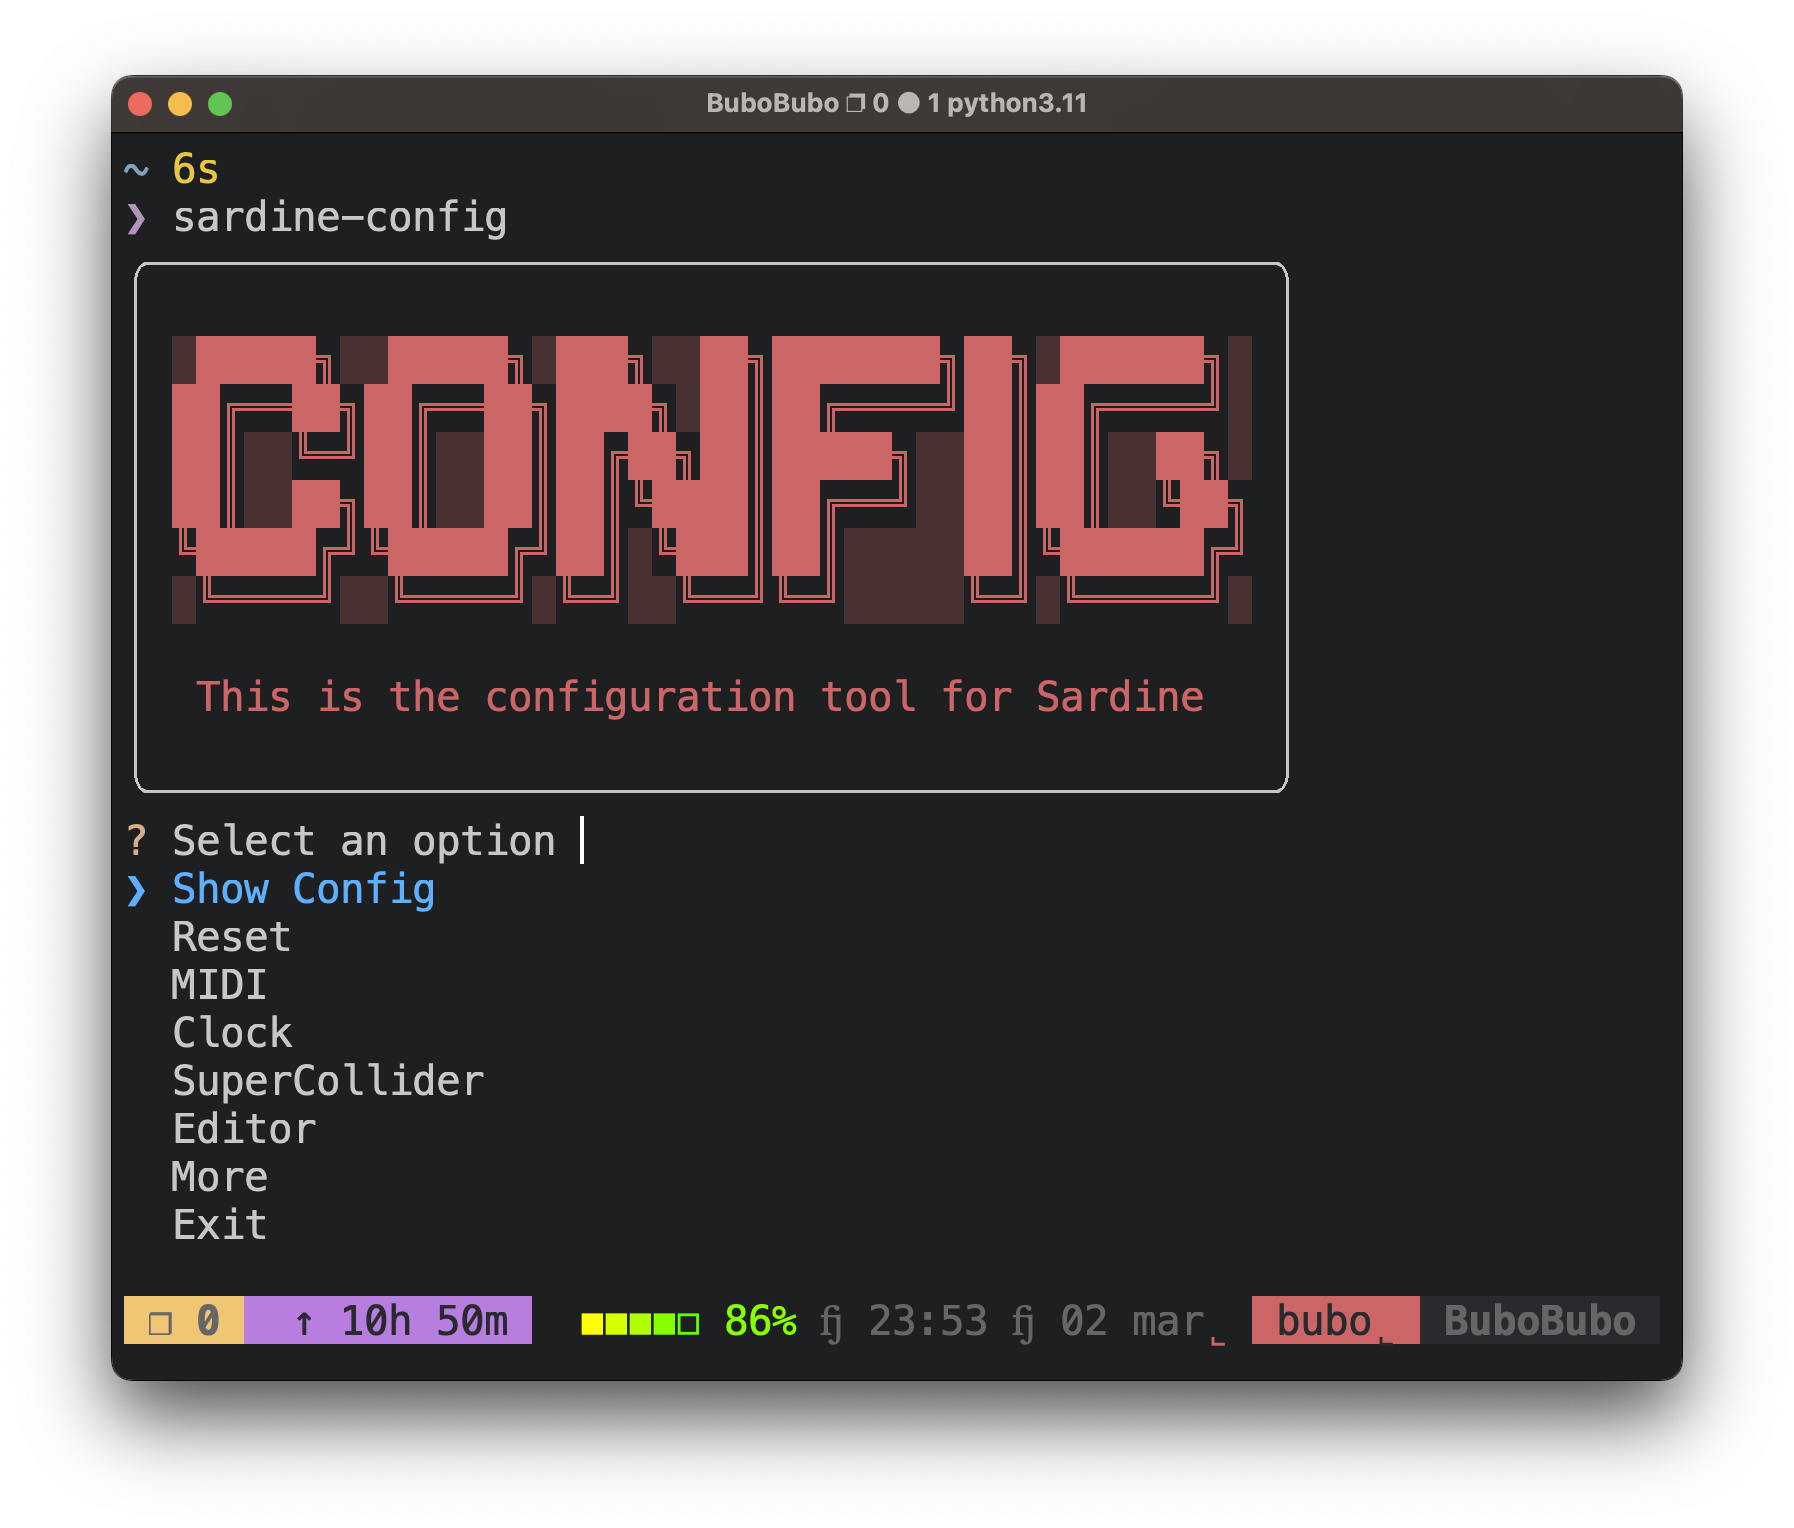
\includegraphics[width=.9\linewidth]{sardine_config.png}
\end{center}

\textbf{Sardine} is shipping its own configuration tool, named \textbf{sardine-config}. Typing \textbf{sardine-config} in your terminal will open a configuration helper tool :) Using it, you can finetune your \textbf{Sardine} experience. Please note that \textbf{Sardine} is writing configuration files to a specific location depending on the OS you are using:
\begin{itemize}
\item \textbf{Windows:}
\item \textbf{MacOS:}
\item \textbf{Linux:}
\end{itemize}

The path leading to the configuration folder can be printed out by typing \texttt{print\_config()} from inside your typical \textbf{Sardine} session. How convenient :) You can also manage to print the \texttt{PATH} to your configuration folder directly from the configuration tool.

There are three main files you can tweak to configure \textbf{Sardine}:
\begin{itemize}
\item \texttt{config.json}: the main configuration file.
\item \texttt{default\_superdirt.scd}: the default configuration for the audio engine.
\item \texttt{user\_configuration.py}: a file that will be runned automatically everytime you start \textbf{Sardine}.
\end{itemize}
There is also a \texttt{synths/} folder (to store synthesizers) and a \texttt{buffers/} folder (used by the web editor).

\subsection{{\bfseries\sffamily TODO} Configuration tour}
\label{sec:orge7d6bd3}

Let's explain what the options in the configuration tool are. To start the configuration tool, please type \texttt{sardine-config} in your terminal. A splashscreen will appear and some options will pop up as well!

\begin{enumerate}
\item Show Config
\label{sec:org3c42e42}

This option will print the configuration file itself. It can be used to double-check if everything is convenably configured.

\item Reset
\label{sec:orgacd9c91}

Reset the configuration file to installation default. This option will only override the \textbf{Sardine} configuration, not the \textbf{SuperDirt} configuration file.

\item MIDI
\label{sec:org65c1223}

The \textbf{MIDI} menu will allow you to select the default \textbf{MIDI} port used by \textbf{Sardine}. This port will be used to automatically create some targets for you to play with when first starting a session. More ports can be configured manually later on.

\begin{itemize}
\item \textbf{Automatic}: \textbf{Sardine} will try to create the.. \textbf{Sardine} virtual port. This only works on \textbf{MacOS} and \textbf{Linux}.
\item \textbf{Manual}: Select a \textbf{MIDI} port from the list. This list is composed of all the MIDI hardware or software ports currently available on your system.
\item \textbf{Custom (advanced)}: write the name of your \textbf{MIDI} port directly. Do not use this except for very good reasons!
\end{itemize}

\item Clock
\label{sec:org5454e73}

This menu will allow you to configure the default clock used by \textbf{Sardine} at the start of a session. You can always switch clock later (even when playing!) but you will usually stick to one clock only for the duration of a session.

\begin{itemize}
\item \textbf{No (internal clock)}: use the system clock. This will not allow you to sync with other players on the local network.
\item \textbf{Yes (external clock)}: use the external Ableton Link clock. This will allow you to synchronize with other players or even with external software supporting the \textbf{Link Protocol}.
\end{itemize}

You will be prompted to enter a new default tempo and a default number of beats per measure.

\item SuperCollider
\label{sec:org9d8d9fc}

\begin{itemize}
\item \textbf{Add SuperDirt Handler}: do you want to interact with \textbf{SuperDirt} at all?! This is different from booting \textbf{SuperCollider}. \textbf{SuperDirt} is a more specialised engine for audio sampling and managing synthesizers. For newcomers, yes, you want to play with \textbf{SuperDirt}!
\item \textbf{Boot a SuperCollider instance}: should \textbf{Sardine} try to manage \textbf{SuperCollider} by itself? This is a safe option to use for people using \textbf{MacOS} or \textbf{Linux} but can result in problems later on for those using \textbf{Windows}.
\begin{itemize}
\item You will have to boot \textbf{SuperCollider} and \textbf{SuperDirt} manually if you untoggle this option!
\end{itemize}
\item \textbf{Use Sardine boot file}: should we load our default boot file?
\item \textbf{Turn on verbose output}: This is a very valuable option to toggle for debugging if \textbf{Sardine} does not work correctly. You will be able to capture the output of the \textbf{SuperCollider} process and see what is wrong on their end :)
\item \textbf{Enter your SuperDirt booth path}: leave blank if you don't know what you are doing.
\end{itemize}

\item Editor
\label{sec:orgb698072}

This menu will allow you to toggle the \textbf{web editor} by default or not. See the section concerning text editors to know if this is an option you want to consider. Note that this option is untoggled by default.

\item More
\label{sec:org521bf3a}

This section is used by developers to add custom debugging options to \textbf{Sardine}.
\end{enumerate}

\subsection{{\bfseries\sffamily TODO} MIDI}
\label{sec:org30dd2a8}

\subsubsection{Receiving MIDI}
\label{sec:org33d65ed}

\textbf{MIDI} Input is supported through the use of a special object, the \textbf{MidiListener} object. This object will open a connexion listening to incoming MIDI messages. There are only a few types of messages you should be able to listen to:

\begin{itemize}
\item \textbf{MIDI} notes through the \texttt{NoteTarget} object
\item \textbf{MIDI} control changes through the \texttt{ControlTarget} object
\end{itemize}

Every MidiListener is expecting a target. You must declare one and await on it using the following syntax:

\begin{verbatim}
a = MidiListener(target=ControlTarget(20, 0))
@swim
def pluck(d=0.25):
    S('pluck', midinote=a.get()).out()
    a(pluck, d=0.25)
\end{verbatim}

In this example, we are listening on the control change n°20 from the default port on the first channel (\texttt{0}). \textbf{Sardine} cannot assert the value of a given \textbf{MIDI} Control before it receives a first message therefore the initial value will be assumed to be \texttt{0}.

You can fine tune your listening object by tweaking the parameters:

\begin{verbatim}
# picking a different MIDI Port
a = MidiListener('other_midi_port', target=ControlTarget(40, 4))
\end{verbatim}

\subsubsection{Sending MIDI}
\label{sec:org341de94}

By default, \textbf{Sardine} will connect to a \textbf{MIDI} port. There is no such thing as a \textbf{Sardine} instance without a link to \textbf{MIDI}. Having only one port means that you will be limited to 16 channels. While this may already be a lot for some, other users will want to do something with their collection of 123 synthesizers. You can manually open up new MIDI ports by tweaking your \textbf{Sardine} session from the \textbf{Python} side:

\begin{verbatim}
# Add a new MidiHandler focusing on a specific port
your_midi_port: str = "exact_name_of_midi_port"
your_midi = MidiHandler(port_name=your_midi_port)

# Add the MIDI port to the session fishbowl
bowl.add_handler(your_midi)
\end{verbatim}

Done! You now have a new MIDI port. The tricky part is now to add new objects to play with! Here is how to do so:

\begin{verbatim}
# If Ziffers is imported, grab a reference to its parser!
if ziffers_imported:
    midi._ziffers_parser = z2

N2 = your_midi.send  # For sending MIDI Notes
PC2 = your_midi.send_program  # For MIDI Program changes
CC2 = your_midi.send_control  # For MIDI Control Change messages
SY2 = your_midi.send_sysex  # For MIDI Sysex messages

if ziffers_imported:
    ZN2 = midi.send_ziffers  # Connecting the new Ziffers parser
#+end_src python

You now have access to an interface to play *notes*, *control changes*, *program changes* and *sysex* messages. If you want to use the shorthand notation, you will have to do one extra step:

#+begin_src python
# Boilerplate for using the newly creating MIDI port with the shorthand
# syntax for swimming functions

def sy2(*args, **kwargs):
    return play(your_midi, your_midi.send_sysex, *args, **kwargs)

def n2(*args, **kwargs):
    return play(your_midi, your_midi.send, *args, **kwargs)

def zn2(*args, **kwargs):
    return play(your_midi, your_midi.send_ziffers, *args, **kwargs)

def cc2(*args, **kwargs):
    return play(your_midi, your_midi.send_control, *args, **kwargs)

def pc2(*args, **kwargs):
    return play(your_midi, your_midi.send_program, *args, **kwargs)
\end{verbatim}

This is everything you need to open new \textbf{MIDI} ports and replicate the normal behavior of the \textbf{Sardine} \textbf{MIDI} port. If you want to go even further, feel free to deep dive into the \texttt{midi} object itself. It might contain some sweet methods that you want to use!

\subsection{{\bfseries\sffamily TODO} OSC}
\label{sec:orgb46b09e}

\textbf{Sardine} is capable of receiving and sending custom \textbf{OSC} messages. Obviously, this should be configured manually on your side. I am only providing the basic tools do to so without encountering any hurdle! Configuring \textbf{OSC} is prone to errors and has always been a very painful activity that computer musicians like to do for some reason.

\subsubsection{Sending OSC}
\label{sec:org055b8a3}

\begin{verbatim}
output_one = OSCHandler(
    ip="127.0.0.1", port=12345,
    name="A first test connexion",
    ahead_amount=0.0, loop=osc_loop, # The default OSC loop, don't ask why!
)
bowl.add_handler(output_one)

output_two = OSCHandler(
    ip="127.0.0.1", port=12346,
    name="A second test connexion",
    ahead_amount=0.0, loop=osc_loop,
)
bowl.add_handler(output_two)

# Look who's here, the send functions as usual
one = output_one.send
two = output_two.send
\end{verbatim}

You can now use the methods one and two as OSC senders just like \texttt{D()} or \texttt{N()}.

\begin{verbatim}
@swim
def one_two_test(p=0.5, i=0):
    """This is a dummy swimming function sending OSC."""
    one('random/address', value='1,2,3')
    again(one_two_test, p=0.5, i=i+1)
\end{verbatim}

If you'd like, you can also make a \texttt{Player} out of it by using the following technique:

\begin{verbatim}
def osc_player(*args, **kwargs):
    """Partial function to add a new OSC player :)"""
    return play(
        output_one,
        output_one.send,
        *args, **kwargs
    )

Pa >> osc_player('random/address', value='1,2,3')
\end{verbatim}

You are now able to send \textbf{OSC} messages just like if they were patterns. It means that you can use the \textbf{Sardine} pattern syntax to compose complex algorithmic sequences of OSC messages. Note that you can also pattern the address, making it a super fun/powerful way to explore your \textbf{OSC} bindings.

\subsubsection{Receiving OSC}
\label{sec:org6a3ce1c}

You can receive and track incoming \textbf{OSC} values coming from your controllers or devices. In fact, you can even attach callbacks to incoming \textbf{OSC} messages and turn \textbf{Sardine} into a soundbox so let's do it!

\begin{verbatim}
# Making a new OSC-In Handler
listener = OSCInHandler(
    ip="127.0.0.1",
    port=44444,
    name="Listener",
    loop=osc_loop
)

# Adding the listener to the bowl
bowl.add_handler(listener)

def funny_sound():
    D('bip', shape=0.9, room=0.9)

listener.attach('/bip/', funny_sound)
\end{verbatim}

That's everything you need! In the above example, we are declaring a new \texttt{OSCInHandler} object that maps to a given \textbf{port} on the given \textbf{IP} address (with \texttt{127.0.0.1} being \texttt{localhost}). All we have to do next is to map a function to every message being received at that address and poof. We now have a working soundbox. Let's break this down and take a look at all the features you can do when receiving OSC.

There are three methods you can call on your \texttt{OSCInHandler} object:

\begin{itemize}
\item \texttt{.attach(address: str, function: Callable, watch: bool)} : attach a callback to a given address. It must be a function. Additionally, you can set watch to \texttt{True} (\texttt{False} by default) to also run the \texttt{.watch} method automatically afterhands.

\item \texttt{.watch(address: str)} : give an address. The object will track the last received value on that address. If nothing has been received yet, it will return \texttt{None} instead of crashing \o/.

\item \texttt{.get(address)} : retrieve the last received value to that address. You must have used \texttt{.watch()} before to register this address to be watched. Otherwise, you will get nothing.
\end{itemize}

\subsection{{\bfseries\sffamily TODO} SuperCollider / SuperDirt}
\label{sec:org75ab131}

The \texttt{default\_superdirt.scd} is\ldots{} your default \textbf{SuperDirt} configuration. \textbf{SuperDirt} is the nickname of a very powerful audio engine used by some live coding libraries like \textbf{Sardine}. By default, this file will specify \textbf{where to look for audio samples} or \textbf{how many inputs and outputs} your system must use.

You must edit it manually if you are willing to change anything to it. This is outside of the reach of \textbf{Sardine} and it is preferable to let the user decide for the most suitable configuration. The \href{https://github.com/musikinformatik/SuperDirt}{SuperDirt} repository is a good place to start, especially the \texttt{hacks/} folder. It will teach you how to edit and configure \textbf{SuperDirt} to your liking. \textbf{SuperDirt} was initially conceived for \href{https://tidalcycles.org/}{TidalCycles}. You will find a great amount of customization options on their website too!

Here is an example showing of how to load more audio samples to play with:

\begin{verbatim}
(
s.reboot {
    s.options.numBuffers = 1024 * 256;
    s.options.memSize = 8192 * 32;
    s.options.numWireBufs = 128;
    s.options.maxNodes = 1024 * 32;
    s.options.numOutputBusChannels = 2;
    s.options.numInputBusChannels = 2;
    s.waitForBoot {
        ~dirt = SuperDirt(2, s);
        ~dirt.loadSoundFiles;
        ~dirt.loadSoundFiles("/Users/bubo/Dropbox/MUSIQUE/LIVE_SMC/DRUMS/*");
        s.sync;
        ~dirt.start(57120, 0 ! 12);
        (
            ~d1 = ~dirt.orbits[0]; ~d2 = ~dirt.orbits[1]; ~d3 = ~dirt.orbits[2];
            ~d4 = ~dirt.orbits[3]; ~d5 = ~dirt.orbits[4]; ~d6 = ~dirt.orbits[5];
            ~d7 = ~dirt.orbits[6]; ~d8 = ~dirt.orbits[7]; ~d9 = ~dirt.orbits[8];
            ~d10 = ~dirt.orbits[9]; ~d11 = ~dirt.orbits[10]; ~d12 = ~dirt.orbits[11];
        );
    };
    s.latency = 0.3;
};
)
\end{verbatim}

SuperDirt treats a wildcard (\texttt{*}) at the end of the path to mean that there are named subdirectories. If you want to load just one sample directory, omit the wildcard.

\section{{\bfseries\sffamily TODO} Text Editor}
\label{sec:orgfbd0163}

Text editors are particularly important to get the most out of \textbf{Sardine}. Remember that this is a tool for \textbf{live coding} and that you will need to setup everything to feel comfortable. \textbf{Sardine} can support most text editors and IDEs. I have been using \textbf{Sardine} using \textbf{Vim}, \textbf{Neovim}, \textbf{Emacs}, \textbf{VSCode} and of course\ldots{} the integrated text editor. This editor is provided mostly for workshops and demos. If you are planning for a gig or anything serious, please consider using and learning a real text editor.

\subsubsection{{\bfseries\sffamily DONE} Fishery Web}
\label{sec:orgba0bbd4}

You don't need a text editor to play with \textbf{Sardine}. Just start the software by typing \texttt{fishery web}. Optionally, you can specify the \texttt{-{}-port} and  \texttt{-{}-???} arguments. Your web browser will promptly open, generally at \texttt{https://localhost:8000}. Your code will automatically be saved in your configuration folder, under the \texttt{buffer/} folder, meaning you can retrieve it later for a new session!

\begin{verbatim}
fishery web
fishery web --port 12345
\end{verbatim}

\begin{center}
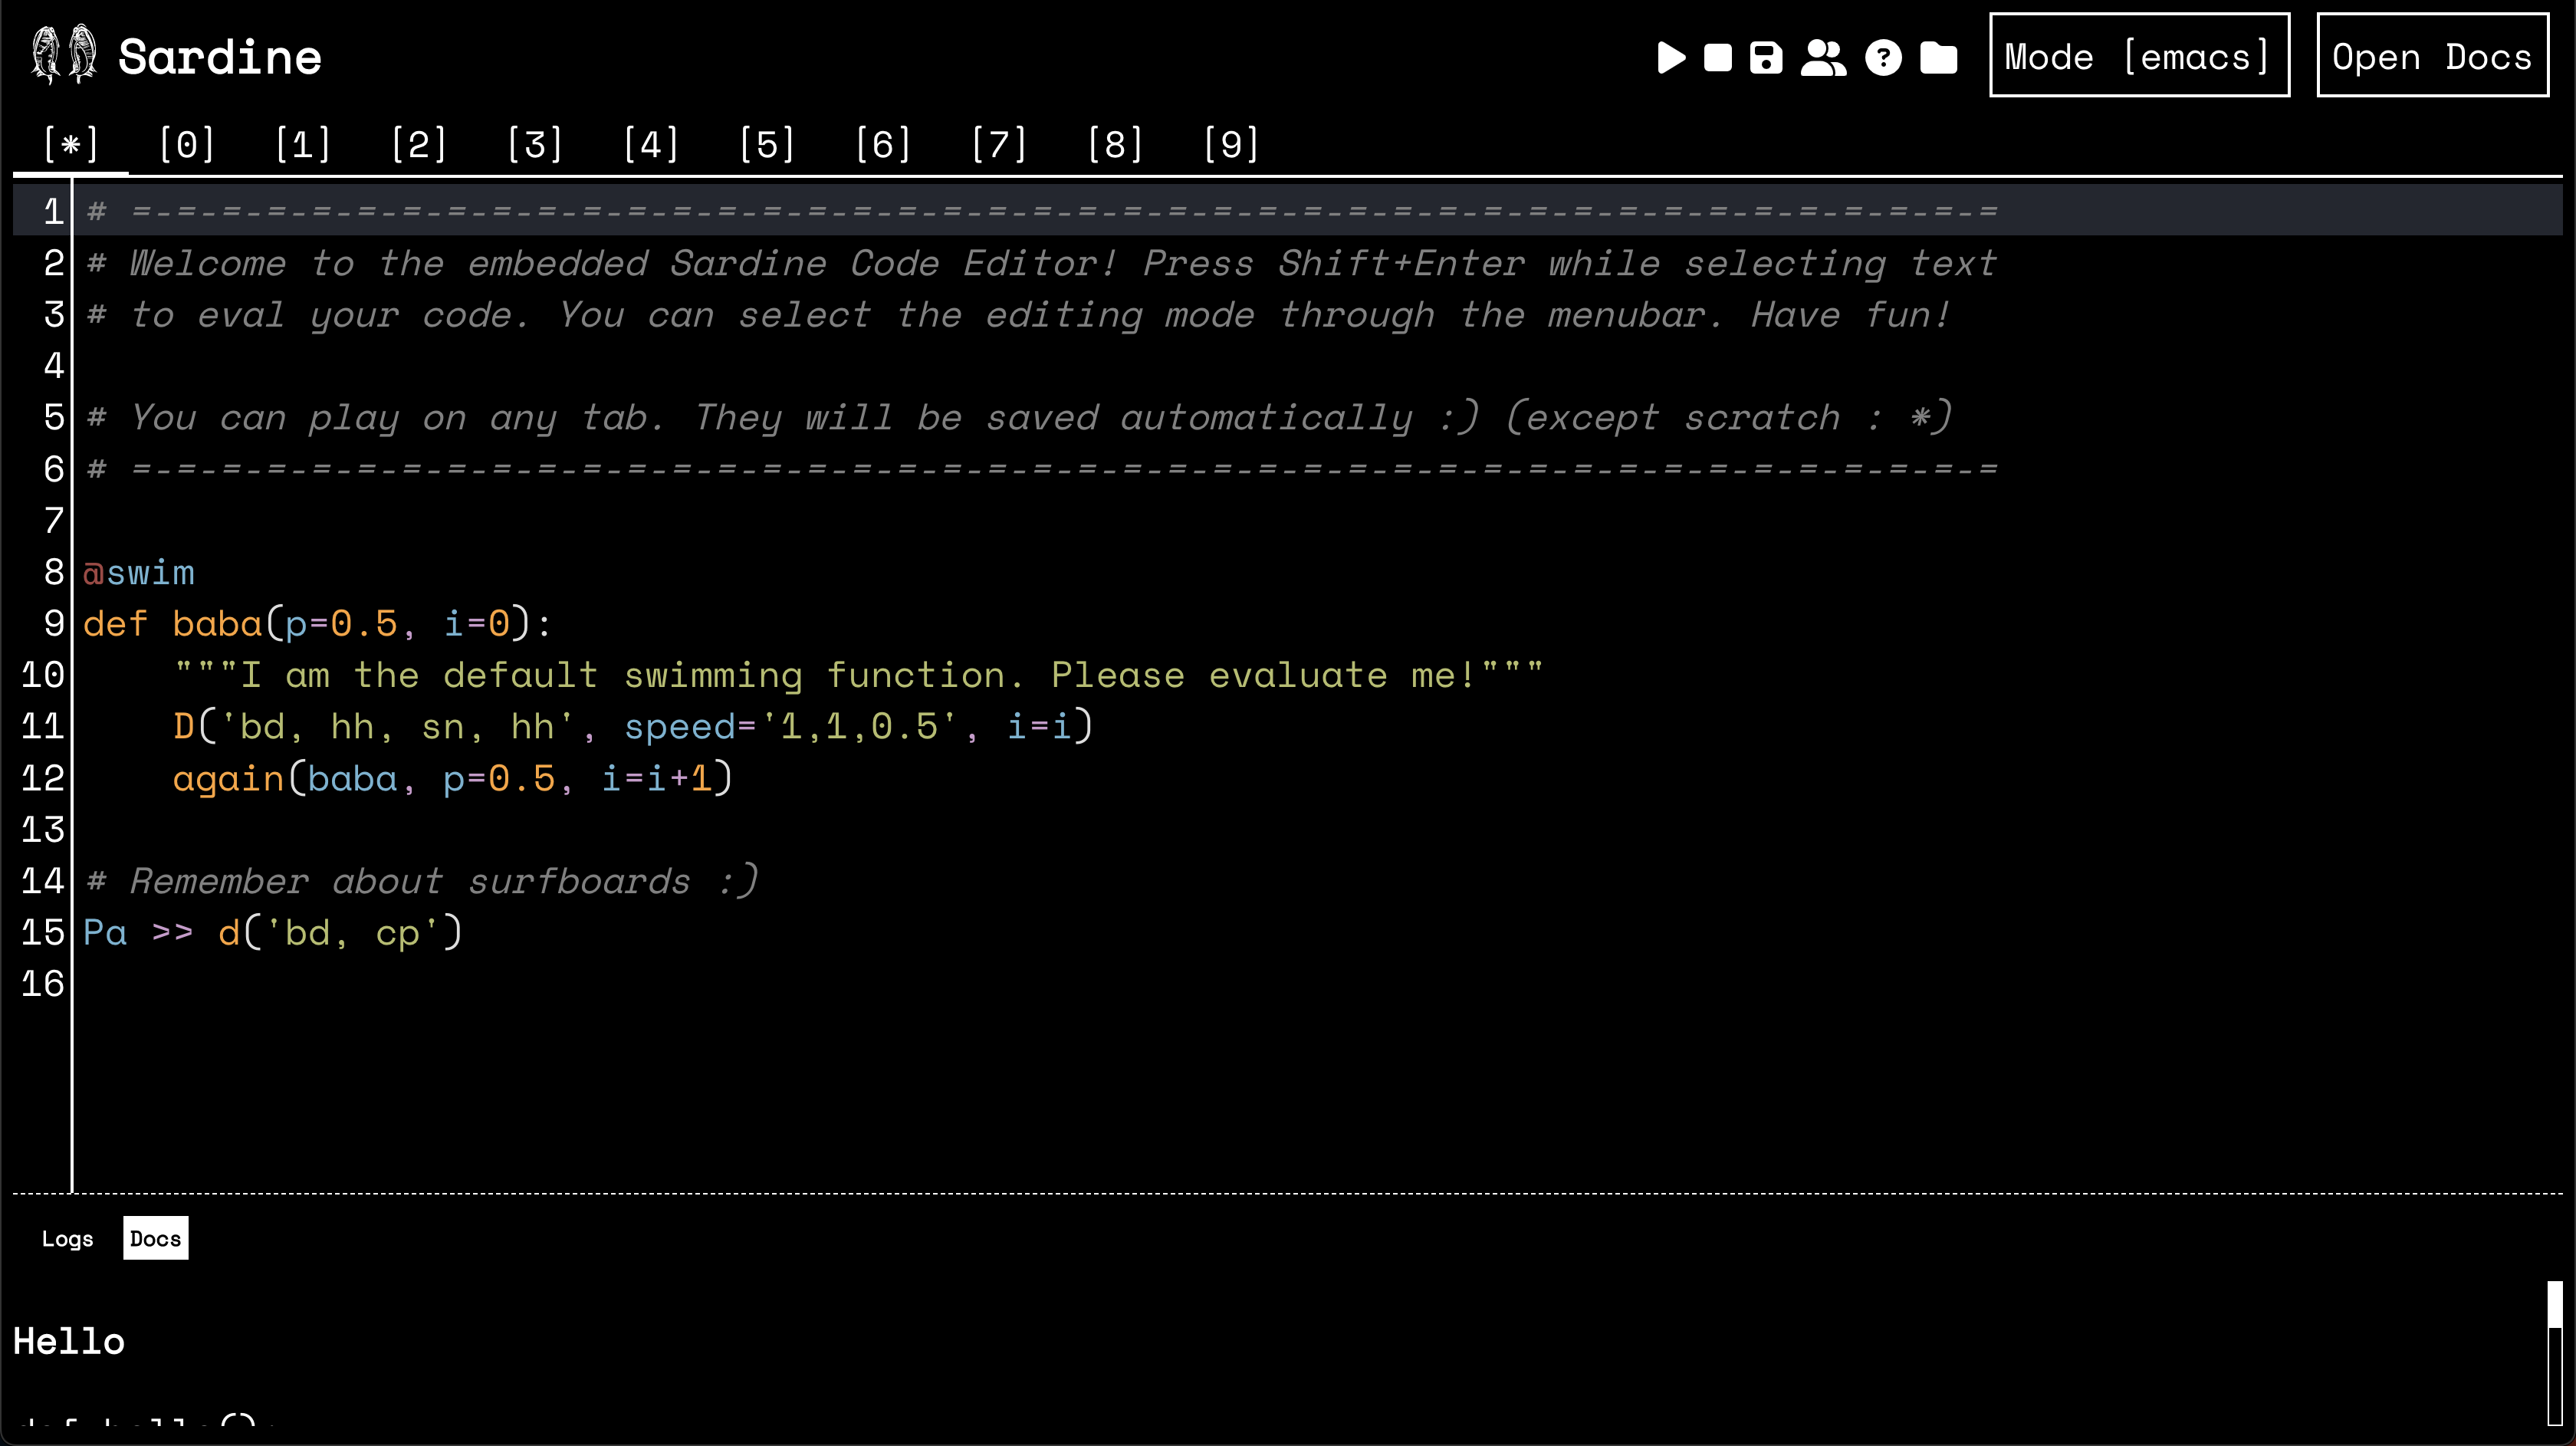
\includegraphics[width=.9\linewidth]{fishery_web.png}
\end{center}

\textbf{Pre v0.2.3 version:} note that you have to manually build the text editor to be able to use it. In the \texttt{/fishery/client} directory, run \texttt{yarn install} and \texttt{yarn run build} to build the text editor. This should only be runned once everytime you install \textbf{Sardine}.

\subsubsection{{\bfseries\sffamily DONE} Flok}
\label{sec:org9e0f09f}

\textbf{Sardine} has been integrated to \href{https://github.com/munshkr/flok}{Flok}, a collaborative text editor for live coding. Using \texttt{Flok}, you can easily share a \textbf{Sardine} session with other musicians and visualists. \texttt{Flok} \textbf{is not an online version of Sardine}. You will still need to install it locally to have sound. However, if you are playing together with some friends in a single room, one only needs to have \textbf{Sardine} installed and active! To use \texttt{Flok}, follow the following instructions:
\begin{itemize}
\item Install \href{https://github.com/munshkr/flok}{Flok} on your computer if you want to use the audio backend (\textbf{Sardine} itself)!
\item Go to \href{https://flok.cc}{flok.cc} or \href{https://sardine.doesnotexist.club}{sardine.doesnotexist} and create a new session by following the prompt.
\item Share the session link with your friends. Use the command to connect your \texttt{REPL} to the session.
\item Have fun!
\end{itemize}

To be 100\% sure that everything will work perfectly, please use \textbf{Firefox}. \textbf{Chrome} has been reported not to work well with \textbf{MacOS}.

\subsubsection{{\bfseries\sffamily TODO} VSCode}
\label{sec:org5f58bed}

\href{https://code.visualstudio.com/}{VSCode} is a powerful and all-devouring code editor developed by \textbf{\textbf{Microsoft}}. It is the most widely spread code editor out there with millions of users, thousands of plugins and corporate support. \textbf{VSCode} is more than capable of handling \textbf{Sardine} sessions and there are multiple ways to configure everything for it.

\begin{itemize}
\item Install the Python support for VSCode using the lateral menu. It might be the first package they will propose you given the popularity of Python!
\item Open up a new terminal using the \texttt{Create new Terminal in the Active Workspace} command (Ctrl/Cmd + Shift + P and search \texttt{>}).
\item Type \texttt{fishery} and press enter to start a new session.
\item Use \texttt{Shift + Enter} to send code to the terminal session.
\end{itemize}

This is a simple yet effective way of using \textbf{Sardine} while retaining all the power of \textbf{VSCode} at your fingertips!

\subsubsection{{\bfseries\sffamily TODO} Vim / Neovim}
\label{sec:org53bba4a}

\textbf{NeoVim} (and by extension \textbf{Vim}) is the editor I currently use on stage but its target audience is mostly developers, old Unix gurus and command-line users. \textbf{Vim} is a modal text editor with multiple modes for editing and jumping around in the source code. It can be extended using plugins and tweaked to your liking. Quite powerful, but it requires some learning to be proficient. The process for working with \textbf{Sardine} from \textbf{Neovim} is pretty straightforward:

\begin{enumerate}
\item install the \href{https://github.com/jpalardy/vim-slime}{slime} plugin.
\begin{itemize}
\item note that the technique to do so might vary depending on your configuration. I am using \href{https://github.com/nanotee/nvim-lua-guide}{Lua} to write my configuration. In the past, I had previously used \href{https://github.com/junegunn/vim-plug}{Plug} for years without encountering any issue!
\end{itemize}
\item split your workspace in two vertical (\texttt{:vs}) or horizontal (\texttt{:sp}) panes.
\item open up a \texttt{:terminal} in one of them and run \texttt{fishery}.
\item work in the other one and use \texttt{C-c C-c} (\texttt{Control+C} twice) to send code from one side to the other.
\begin{itemize}
\item \textbf{slime} will probably ask you which job to target, just press enter!
\end{itemize}
\end{enumerate}


\subsubsection{{\bfseries\sffamily TODO} (Doom) Emacs}
\label{sec:org7fd1ccd}

I am using \textbf{Doom Emacs} for many things in my life: writing this documentation, writing manuscripts and papers and.. playing some music with \textbf{Sardine}. The venerable \textbf{Emacs} is -- of course -- able to manage \textbf{Sardine}! Please use the \texttt{python.el} plugin. This mode will allow you to pipe easily your code from a text buffer to a running interpeter. The plugin is adding quality-of-life features for working with \textbf{Python} in general but also makes working with a \textbf{REPL} much easier and much more convenient. If you are new to the vast world of \textbf{Emacs}, it is probably worthwhile to take a look at \href{https://github.com/doomemacs/doomemacs}{Doom Emacs} or \href{https://github.com/syl20bnr/spacemacs}{Spacemacs}, both being equally great. I will not dive into more details. If you are able to configure \textbf{Emacs}, you will be able to configure your editor for \textbf{Sardine} :).

The following code is the one I use for running \textbf{Sardine} using \textbf{Doom Emacs}. It is not great and I should probably make something cleaner or even create a dedicated package for \textbf{Sardine} but life is short, and nobody is writing the docs while I finetune my \textbf{Emacs} config.

\begin{verbatim}
;; =-=-=-=-=-=-=-=-=-=-=-=-=-=-=-=-=-=-=-=-=-=-=-=-=-=-=-=-=-=-=-=-=-=
;; SARDINE MODE
;; =-=-=-=-=-=-=-=-=-=-=-=-=-=-=-=-=-=-=-=-=-=-=-=-=-=-=-=-=-=-=-=-=-=
;; Customize the python-mode to run Sardine code using the terminal.

(setq
 python-shell-interpreter "fishery"
 python-shell-interpreter-args "")

(defun sardine/start-sardine ()
  "Start a new interactive Sardine Session"
  (interactive)
  (run-python))

(defun sardine/eval-block ()
  "Evaluate a sardine code block"
  (interactive)
  (mark-paragraph)
  (if (and transient-mark-mode mark-active)
      (python-shell-send-region (point) (mark))
    (python-shell-send-region (point-at-bol) (point-at-eol)))
  (forward-paragraph))

(defun sardine/stop-code ()
  "Stop all the Sardine code currently running"
  (interactive)
  (python-shell-send-string "panic()"))

; Unmapping keys from the Python mode
(add-hook 'python-mode-hook
          (lambda() (local-unset-key (kbd "C-c C-c"))))
(add-hook 'python-mode-hook
          (lambda() (local-unset-key (kbd "C-c C-s"))))

; Remapping keys
(global-set-key (kbd "C-c C-c") #'sardine/eval-block)
(global-set-key (kbd "C-c C-s") #'sardine/stop-code)
\end{verbatim}

\subsubsection{{\bfseries\sffamily TODO} Others}
\label{sec:orgbe471dc}


In the past, people have been running \textbf{Sardine} code on many different text editors and platforms:
\begin{itemize}
\item \href{https://jupyter.org}{Jupyter Notebook}: a very popular framework for using \textbf{Python} in data sciences, machine learning, etc.
\item \href{https://github.com/atom}{Atom} (\textbf{depracated}) / \href{https://pulsar-edit.dev/}{Pulsar}: killed by \textbf{Microsoft}, was once a very nice but slow text editor/IDE.
\end{itemize}

We know this is working, but there is no documentation about it or the one we have is outdated!

\section{{\bfseries\sffamily TODO} Basics}
\label{sec:org265a6d7}
\subsection{{\bfseries\sffamily TODO} Time}
\label{sec:org7c6bfd0}
\subsection{{\bfseries\sffamily TODO} Pattern}
\label{sec:org17a2973}
\section{About}
\label{sec:org615194e}
\subsection{Why Sardine?}
\label{sec:org4a3d22c}

\textbf{Sardine} is a side-project that initially started as an attempt to demonstrate some live coding techniques for my PhD dissertation in musicology at the University of Saint-Etienne / Paris 8 University. \textbf{Sardine} is trying to encompass various programming paradigms and gestures used by live coders: declarative and imperative programming, DSLs for pattern processing, clock synchronisation with other tools, etc. Initially, everything was working according to the plan. And then, the tool started mutating from all sides and it gained its own identity. It is now a new live coding library in need of support :)

Obviously, I'm also trying to develop \textbf{Sardine} for my friends and I. Programming new tools is fun and rewarding! I am playing music with the \href{https://cookie.paris/}{Cookie Collective} in Paris and with the \href{https://discord.gg/arRBSfdXV3}{Creative Code Lyon} community. I am also very much attached to the values of the \href{https://toplap.org/}{TOPLAP} collective once was contributing to the documentation of \href{https://tidalcycles.org/}{TidalCycles}. Live coding is a fun musical practice, that I nowadays consider very much alike playing a different kind of musical instrument!

I learned how to program by live coding music! The next logical step I could see in my learning was to code my own tool so I can share it with others and make people see the incredibly fruitful intersection between code and music. Since I started live coding a few years ago, I always wished to develop my own tool just to see how things work! I am now finding the need to write documentation for my own work.. heh\ldots{}

\subsection{Contributions}
\label{sec:orgd2fd39c}

Contributions of any sort are really welcome! I am not a professional developer and am just trying to do my best with \textbf{Sardine}! I might code things in a weird or unefficient way. Everything takes place on the main \href{https://github.com/Bubobubobubobubo/sardine}{GitHub} repo. Don't be afraid of proposing drastic changes or to take a different direction from mine! I'm here for the fun!
\end{document}